\chapter{图神经网络}
\label{chap:graph-networks}

一个分子可以有不同数量的原子，每个原子连接的化学键也不一样；一篇论文的类别除了取决于正文，还可能与它引用的论文有关。这些输入既没有图像中整齐的网格，也没有序列中唯一的先后次序。若把对象按编号拼成向量，同一分子只需换一种原子编号，网络就会读到另一个输入；若只对每个对象单独使用前馈网络，又会丢掉连接关系。本章要回答的问题是：网络怎样利用不规则的关系形成表示，同时让预测遵守对象重编号及任务本身的对称性？

这个问题需要同时考察计算规则和信息范围。节点从哪些邻居读取信息、怎样把数量可变的输入组合起来，决定一轮计算；传播多少轮、是否反复使用同一组参数，决定关系影响能够传多远。关系的类型、变化时间和几何含义又会约束消息的形式。我们从共同的消息传递结构出发，比较不同图卷积与循环更新，再检查表示区分能力、传播行为和泛化条件，最后把这些选择接到具体预测任务中。

\section{图神经网络概述}
\label{sec:gnn-overview}

前馈网络可以处理预先提取的分子描述向量，但描述向量中包含什么关系，取决于特征设计。卷积网络共享一个窗口内的计算，依赖网格中明确的相对位置；一般关系网络没有统一的“左上邻居”。循环网络能够读取一串对象，却需要额外规定遍历次序。序列化和固定特征仍然可以用于图任务，只是这些表示需要另行解决关系保留、长度变化和编号敏感的问题。

沿用\BookSectionRef{sec:graph-theory-objects-representations}{第一卷“数学准备”的图对象与表示节}，
记输入关系为$\mathcal G=(V,E)$，$V=\{1,\ldots,n\}$，$e=|E|$。
节点$i$的属性为$\bm x_i\in\mathbb R^d$，消息边$j\to i$的属性记为$\bm a_{i,j}\in\mathbb R^{d_e}$。
消息下标先写接收者，再写发送者；它不是卷一的有向边起点、终点排列。
分子属性可包含原子与键类型，引用网络的属性可包含论文内容。

卷一的有向邻接矩阵以行记起点、列记终点。本章为直接写出接收端汇总，使用其转置
$\bm A=\bm A_{\mathrm{graph}}^\top$，因此$\bm A_{i,j}$为$j\to i$的权重。
$N(i)=\{j:\bm A_{i,j}\ne0\}$是发送有效消息的入邻域；
零权结构边若仍需参与计算，应另存结构掩码。无向图上矩阵对称，两种表示相同。
后文的谱域推导采用非负权重无向图，基础消息传递允许有向边。

\term{图神经网络}（graph neural network, GNN）让网络沿给定关系交换并组合对象的表示。它把“谁与谁相连”变成计算的组织依据，共享的更新规则则使同一网络可以处理不同节点数和邻居数。图在这里表示输入关系；它不自动表示概率模型中的条件独立性，也不意味着每条边都是因果关系。

编号只是保存节点的方式，不能改变节点本身的含义。令$\bm{X}\in\mathbb{R}^{n\times d}$按行存放节点特征，即$\bm{X}_{i,:}=\bm{x}_i^{\top}$；用\term{置换矩阵}（permutation matrix）$\bm{P}$重新排列这些行，则新的输入为$\bm{X}'=\bm{P}\bm{X}$、$\bm{A}'=\bm{P}\bm{A}\bm{P}^{\top}$，边属性也须同步重排。\term{置换等变性}（permutation equivariance）要求节点输出跟着节点一起重排；\term{置换不变性}（permutation invariance）要求整图输出保持不变。不含边属性时，两种要求可写为
\begin{equation}
  \begin{aligned}
    F(\bm{P}\bm{A}\bm{P}^{\top},\bm{P}\bm{X})
      &=\bm{P}F(\bm{A},\bm{X}),\\
    f(\bm{P}\bm{A}\bm{P}^{\top},\bm{P}\bm{X})
      &=f(\bm{A},\bm{X})\text{。}
  \end{aligned}
  \label{eq:gnn-permutation}
\end{equation}
$F$产生按节点排列的输出，$f$产生整图输出。重编号后，每个原子的预测仍对应同一个原子，分子的属性预测仍对应同一个分子；等变性并不要求不同原子的输出相同。

沿关系学习表示的思想早于今天的图卷积层。早期处理树和有向无环结构的递归网络，沿既定依赖逐步形成表示；一般图中的环却使“等邻居算完再计算自己”缺少自然终点。Gori等在2005年提出图神经网络模型，将节点状态定义为相互依赖方程的解，允许直接处理带环的图，并区分节点任务与整图任务\scite{gori2005graphdomains} Scarselli等在2009年的系统论述中，以共享局部更新和收缩条件保证状态解唯一，再通过反复更新求得稳定状态。这条路线的核心是让关系参与表示形成，同时使带环依赖能够求值；收缩条件也限制了可选的更新函数\scite{scarselli2009gnn}

另一条路线试图把卷积网络的共享滤波推广到不规则结构。Bruna等在2014年的Spectral CNN中，用图拉普拉斯的特征向量替代普通傅里叶模式，在这些模式上学习滤波响应。它给出了图卷积的谱域定义，但显式特征基带来计算成本和跨图使用的困难\scite{bruna2014spectral} Defferrard等在2016年以切比雪夫多项式实现谱滤波，使计算转为有限邻域上的稀疏传播，无需显式求出完整特征基。这里改变的不只是计算速度：多项式同时明确了滤波器能够读取多远的关系\scite{defferrard2016chebnet}

到2016至2017年，图上的有限轮次计算形成了几种不同设计。门控图网络用门控状态更新替代必须迭代至不动点的求值方式；GCN把谱滤波的低阶近似改写为简单的归一化邻域层，便于用节点标签端到端训练；GraphSAGE通过采样与共享聚合，为大图和未见节点组织计算。这些模型分别改变了状态求值、传播算子和邻域读取方式，不是一条只靠增加层数的发展线索。后文将展开相应机制与条件。

这些设计又需要共同语言来比较。Gilmer等在2017年把许多分子图模型概括为消息计算、状态更新和整图读出，使节点、边属性及参数共享的位置能够明确对照\scite{gilmer2017mpnn} 随后的问题从“能否沿边计算”转向“应保留哪些差别”：2018年的GAT用内容决定邻居权重，2019年的GIN联系邻域聚合与图结构区分能力。相关研究还将状态扩展到多种关系、随时间出现的事件及带几何坐标的对象，并分析传播过深时的信息损失。这些方向共同说明，图网络的发展既关心计算规模，也关心关系语义、对称性与表示能力。

因此，基础、卷积和循环图网络不是三套彼此隔绝的机制。基础结构回答如何沿边传递信息；卷积模型进一步规定传播算子；循环模型强调同一更新规则反复作用于状态。图的边可以形成环，但固定轮次展开后的计算图仍沿轮次前进，能够使用前面章节的反向传播。

\section{基础图神经网络}
\label{sec:gnn-basic}

要让一个节点利用邻居，既要把邻居的属性变成可用信息，也要处理邻居数量不一致的问题。若把邻居按编号拼接，输入宽度会变化，计算还会依赖拼接次序。把各条边上的计算与邻域组合分开，可以同时解决这两个问题。

\subsection{网络结构}
\label{sec:gnn-structure}

\term{消息传递}（message passing）指每个节点沿边接收邻居提供的信息，再据此更新自身表示。消息是可学习的数值向量，不要求系统实际发送一条通信消息。用$\bm{h}_i^{(l)}\in\mathbb{R}^{m_l}$表示节点$i$在第$l$轮之后的隐表示，初态可取$\bm{h}_i^{(0)}=\phi_{\mathrm{in}}(\bm{x}_i)$。一轮计算由三个步骤组成：
\begin{equation}
  \begin{aligned}
    \bm{m}_{i\leftarrow j}^{(l)}
      &=M^{(l)}\!\left(\bm{h}_i^{(l)},\bm{h}_j^{(l)},\bm{a}_{i,j}\right),\\
    \overline{\bm{m}}_i^{(l)}
      &=\operatorname{AGG}^{(l)}
        \!\left(\{\!\{\bm{m}_{i\leftarrow j}^{(l)}:j\in N(i)\}\!\}\right),\\
    \bm{h}_i^{(l+1)}
      &=U^{(l)}\!\left(\bm{h}_i^{(l)},\overline{\bm{m}}_i^{(l)}\right)\text{。}
  \end{aligned}
  \label{eq:gnn-message-passing}
\end{equation}
$M^{(l)}$是消息函数，输出固定维度的消息；$\operatorname{AGG}^{(l)}$是聚合函数，把任意数量的消息组合成一个固定维度的向量；$U^{(l)}$是节点更新函数。双花括号表示\term{多重集合}（multiset）：其中元素没有顺序，但重复出现的次数仍然有意义。两个邻居具有相同状态时，求和应计入两次，而不能因为数值相同就丢掉一个。

聚合通常选求和、平均或逐坐标最大值，也可以先计算权重再加权求和。空邻域上的求和取零；平均和最大值需要另约定空输入，例如取零并提供空邻域标记。另一种做法是加入\term{自环}（self-loop），使节点也向自身发送消息。自环是否与普通边共享参数取决于模型，不能在已包含自身的更新中无说明地重复计入。

图~\ref{fig:gnn-message-passing}把节点$i$的一轮计算展开。各邻居先通过同一消息函数，再进入对次序不敏感的聚合；节点自己的旧表示另进入更新。这种分工既容纳边属性，也保留自身与邻居信息的区别。
\begin{figure*}[htb]
  \centering
  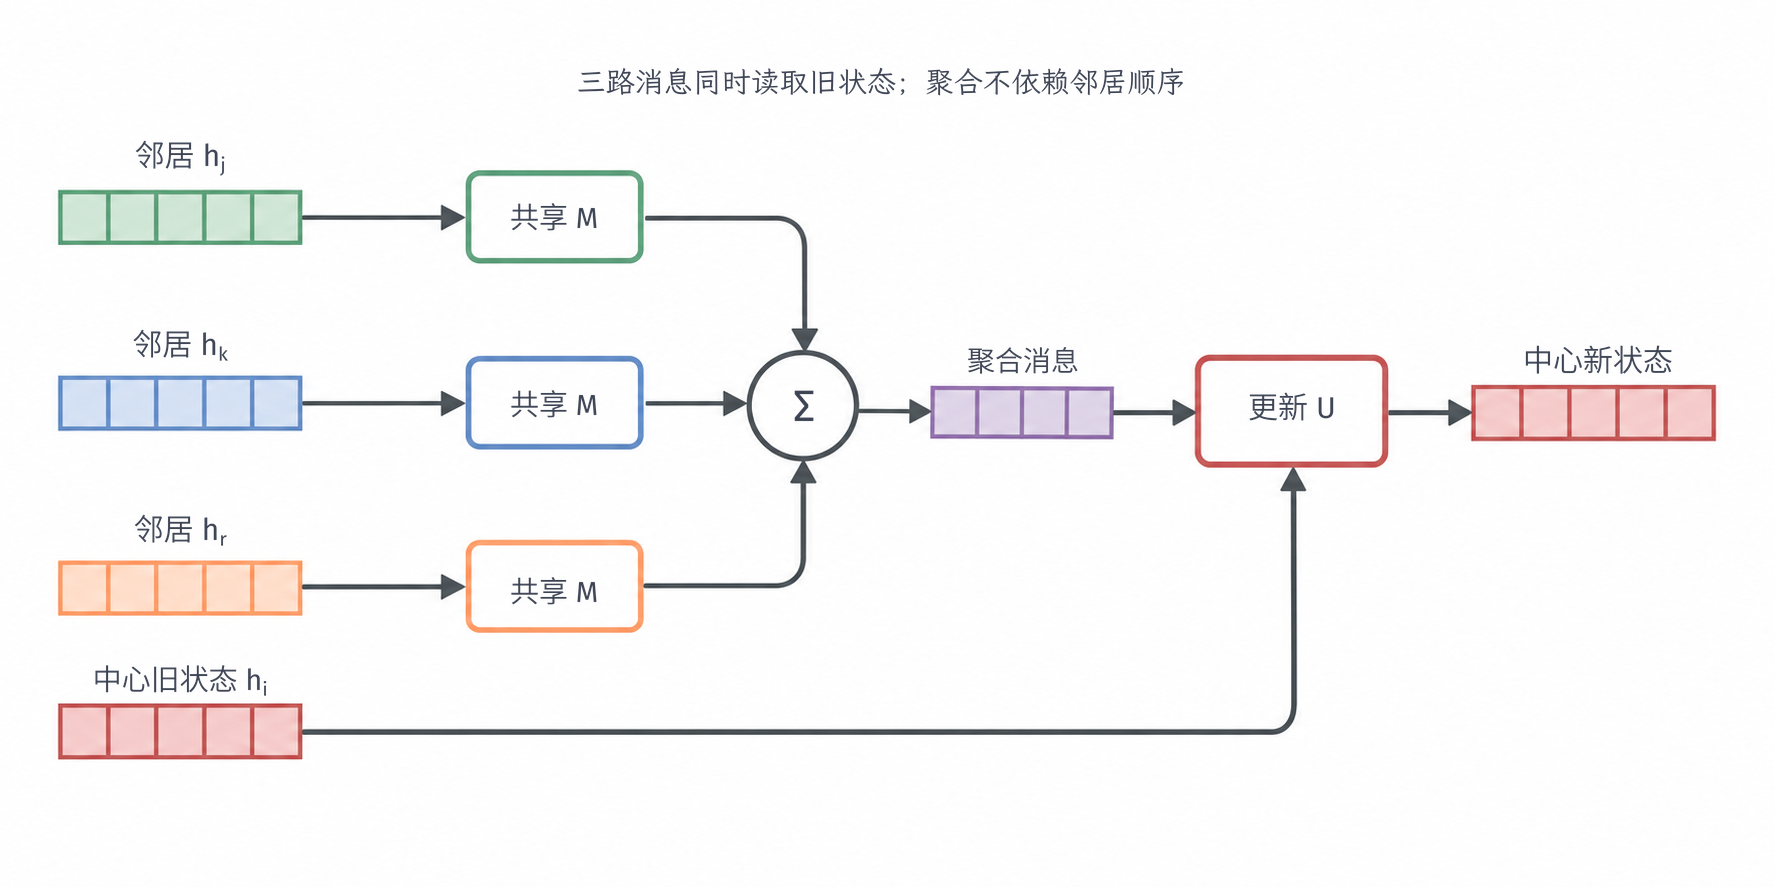
\includegraphics[width=\linewidth]{figures/03-models/02-neural-network-models/generated/gnn-message-passing/figure.png}
  \caption{节点$i$的一轮消息传递。左侧三行邻居表示分别产生消息，经求和聚合后更新节点$i$。下方独立路径把$i$的旧表示送入更新函数。图中省略消息函数对接收节点和边属性的额外输入，所有节点使用相同的消息与更新规则。}
  \label{fig:gnn-message-passing}
\end{figure*}

在同一轮内，$M^{(l)}$和$U^{(l)}$的参数在所有节点与边上共享。因此，增加节点会增加计算量，却不必增加参数量。若邻域聚合不依赖枚举次序，输入编码和节点更新也使用共享函数，就可按轮归纳证明式\eqref{eq:gnn-permutation}：重编号只重排消息的接收位置，聚合结果跟着重排，更新后的表示也跟着重排。随机邻居采样还要求采样规则与编号无关；不同随机抽样下输出数值未必一致，等变性应针对对应的抽样或输出分布理解。

一轮只能读取直接邻居的旧表示。两轮之后，邻居的表示已经包含它们的邻居，节点因而可以利用两跳以内的信息。\term{图上的感受野}（graph receptive field）就是能够经传播影响当前表示的节点范围；在仅使用一跳邻域、没有全局通路时，$L$轮的范围至多为$L$跳。图~\ref{fig:gnn-propagation}强调更新的同步性：必须读完上一轮再写下一轮，不能把本轮刚更新的状态混入其他节点的同轮输入。

\begin{figure*}[htb]
  \centering
  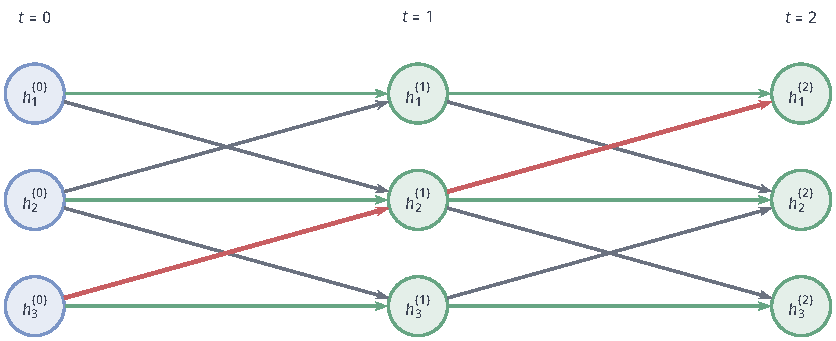
\includegraphics[width=\linewidth]{figures/03-models/02-neural-network-models/tikz/gnn-propagation/figure.pdf}
  \caption{三节点路径上的同步传播。列顶的$t=0,1,2$表示同步快照，横向实线传递自身状态，斜线沿原图的相邻关系传递状态。红色粗线描出节点3经节点2影响节点1的两跳路径；同一列内没有即时传播，因此一次更新不能直接读取两跳之外的新信息。}
  \label{fig:gnn-propagation}
\end{figure*}

\begin{example}[两轮邻域平均]
\label{ex:gnn-two-rounds}
取无向路径$1-2-3$，初始标量为$\bm{x}=(1,0,2)^{\top}$。为单独观察传播，暂不使用可学习参数与非线性，令
\[
  h_i^{(l+1)}=\frac{h_i^{(l)}+\sum_{j\in N(i)}h_j^{(l)}}{1+|N(i)|}\text{。}
\]
一轮结果为$(1/2,1,1)^{\top}$，两轮结果为$(3/4,5/6,1)^{\top}$。节点1在第一轮没有读取节点3，第二轮却通过节点2受到节点3的影响。这是人为构造的传播例子，不是训练所得的实验结果。
\end{example}

节点表示形成后，整图预测还需要\term{读出}（readout）：把数量可变的节点表示变成一个图表示。基本形式是
\begin{equation}
  \bm{g}=\rho\!\left(\sum_{i\in V}\phi(\bm{h}_i^{(L)})\right),
  \qquad \widehat{\bm{y}}=g_{\mathrm{out}}(\bm{g})\text{，}
  \label{eq:gnn-readout}
\end{equation}
其中$\phi$是共享的节点变换，$\rho$是聚合后的变换。求和不因节点重排而改变，所以它把节点等变表示转为整图不变表示。平均会消去部分规模信息，最大值强调是否出现某类特征；若目标随对象数量累积，求和更符合这一结构假设，但仍需验证目标是否具有相应可加性。

只计固定宽度$m$下的稠密线性节点变换和线性消息，一轮常可组织为$O(nm^2+em)$：先对节点变换，再沿边聚合。若每条边都单独通过宽度为$m$的稠密网络，边计算可以达到$O(em^2)$。因此，“图网络计算量随边数增长”需要同时说明消息函数和特征宽度。训练还要保存多轮激活；可变节点数不会自动带来固定的训练存储量。

\subsection{输出和学习目标}
\label{sec:gnn-output-objectives}

预测对象可以是节点、节点对或整张图。三者可以共享同一个图编码器，但监督位置和样本组织不同。图~\ref{fig:gnn-output-levels}把这三种读出对应起来；损失仍按第~\ref{sec:ffn-output-objectives}节所介绍的输出含义选择。

\begin{figure*}[htb]
  \centering
  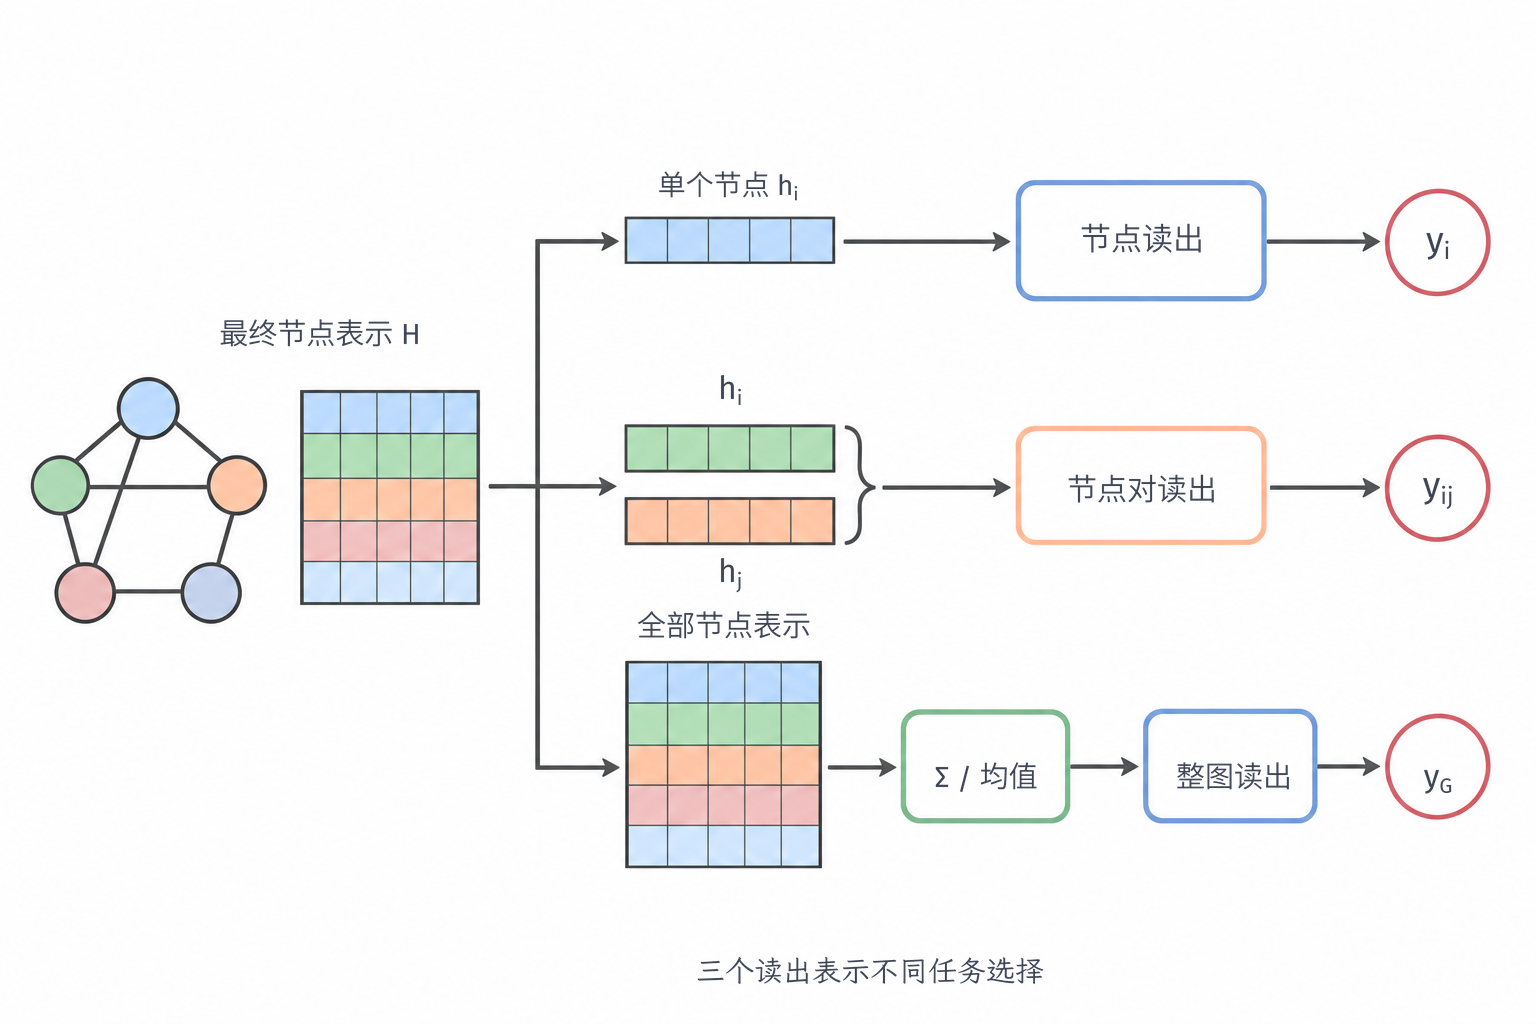
\includegraphics[width=\linewidth]{figures/03-models/02-neural-network-models/generated/gnn-output-levels/figure.png}
  \caption{同一组节点表示的三种任务读出。三个分支分别承载节点、节点对和整图任务，并在相应位置执行读出。节点预测读取一个节点，边或连接预测读取两个端点及可用的关系属性，整图预测先对全部节点作对称聚合；三个分支不要求在同一模型中同时启用。}
  \label{fig:gnn-output-levels}
\end{figure*}

节点分类在每个受监督节点上计算类别概率。设类别数为$C$，标签$y_i\in\{1,\ldots,C\}$，训练标签所在节点集合为$V_{\mathrm{train}}$，则
\begin{equation}
  \begin{aligned}
    \bm{p}_i&=\operatorname{softmax}(\bm{W}_{\mathrm{out}}\bm{h}_i^{(L)}+\bm{b}_{\mathrm{out}}),\\
    L_{\mathrm{node}}&=-\frac{1}{|V_{\mathrm{train}}|}
      \sum_{i\in V_{\mathrm{train}}}\log p_{i,y_i}\text{。}
  \end{aligned}
  \label{eq:gnn-node-loss}
\end{equation}
$\bm{W}_{\mathrm{out}}\in\mathbb{R}^{C\times m_L}$，$\bm{b}_{\mathrm{out}}\in\mathbb{R}^{C}$。其他节点可以按设定参与消息传递，但它们的标签不因此成为训练输入。标签掩码决定损失的位置，不能只把测试标签乘零后留在输入特征中。

边预测需要同时读取端点。设候选节点对集合为$B$，用成对读出函数计算得分，再变成存在连接的预测概率：
\[
  \begin{aligned}
    s_{i,j}&=g_{\mathrm{pair}}(\bm{h}_i^{(L)},\bm{h}_j^{(L)},\bm{a}_{i,j}),\\
    p_{i,j}&=\operatorname{sigmoid}(s_{i,j})\text{。}
  \end{aligned}
\]
对二值目标$b_{i,j}$可使用
\begin{equation}
  L_{\mathrm{edge}}=-\frac{1}{|B|}\sum_{(i,j)\in B}
    \left[b_{i,j}\log p_{i,j}+(1-b_{i,j})\log(1-p_{i,j})\right]\text{。}
  \label{eq:gnn-edge-loss}
\end{equation}
未观察到的连接通常没有该边的属性，此时应省略属性或使用预测时可得的候选关系类型。无向连接的评分需要满足$s_{i,j}=s_{j,i}$，例如采用点积；有向连接可以使用一般双线性评分或有序拼接，不能用对称评分表达任意方向差异。

整图预测把第$q$张图的读出$\bm{g}_q$映射为类别或数值，按独立图样本平均损失。回归目标$y_q\in\mathbb{R}$可写为
\begin{equation}
  L_{\mathrm{graph}}=\frac{1}{N}\sum_{q=1}^{N}
    \left(g_{\mathrm{out}}(\bm{g}_q)-y_q\right)^2\text{，}
  \label{eq:gnn-graph-loss}
\end{equation}
其中$N$是训练图数，各图的节点数$n_q$可以不同。按图平均给每张图相同权重；按全部节点平均会改变大图与小图的相对权重，二者对应不同的经验目标。

\subsection{参数学习}
\label{sec:gnn-learning}

\subsubsection{沿消息通路回传梯度}
\label{sec:gnn-message-backprop}

固定$L$轮时，式\eqref{eq:gnn-message-passing}是有限的函数复合。前向沿边$j\to i$读取节点$j$的状态，反向则计算这份状态对节点$i$的预测误差有多大影响，再把相应导数回到$j$。这条反向依赖不要求原图另有一条$i\to j$的边；它来自前向计算的链式法则。图中的环已沿传播轮次展开，反向依次处理$l=L-1,\ldots,0$，不会在同一轮内无限绕圈。

用列向量$\bm{g}_i^{(l)}=\partial L/\partial\bm{h}_i^{(l)}\in\mathbb{R}^{m_l}$记节点状态的总梯度。节点分类的输出头在受监督节点产生初始梯度；整图读出把整图损失回传到参与读出的节点；连接预测的评分头向两个端点回传。没有自身标签的节点也可能因影响其他节点的预测而得到梯度。下面暂设损失只经最终轮状态产生，若中间轮也有输出，须在该轮另加直接损失的导数。

一轮反向计算可以对应前向的三个环节。令消息宽度为$r_l$，聚合宽度为$\overline r_l$，先将$\bm{g}_i^{(l+1)}$经更新函数回到聚合向量，再经聚合回到各条消息：
\begin{equation}
  \begin{aligned}
    \bm{v}_i^{(l)}
      &=\left(\frac{\partial U^{(l)}}
        {\partial\overline{\bm{m}}_i^{(l)}}\right)^{\top}
        \bm{g}_i^{(l+1)},\\
    \bm{\delta}_{i\leftarrow j}^{(l)}
      &=\left(\frac{\partial\operatorname{AGG}^{(l)}}
        {\partial\bm{m}_{i\leftarrow j}^{(l)}}\right)^{\top}
        \bm{v}_i^{(l)}\text{。}
  \end{aligned}
  \label{eq:gnn-message-adjoints}
\end{equation}
这里$\bm{v}_i^{(l)}\in\mathbb{R}^{\overline r_l}$，$\bm{\delta}_{i\leftarrow j}^{(l)}\in\mathbb{R}^{r_l}$；两个局部Jacobian矩阵的形状分别为$m_{l+1}\times\overline r_l$和$\overline r_l\times r_l$。所有导数都在前向保存的状态、消息及参数上计算。求和聚合的Jacobian是单位矩阵，所以每条消息收到同一个$\bm{v}_i^{(l)}$；平均聚合再除以邻居数；逐坐标最大值把导数送到被选中的位置，平局处需约定次梯度或记录规则。内容相关加权还要对权重求导，不能只按固定加权和回传。

消息函数的两个状态输入会产生不同贡献。记$\bm{J}_{1,i,j}^{(l)}$、$\bm{J}_{2,i,j}^{(l)}\in\mathbb{R}^{r_l\times m_l}$分别为$M^{(l)}$关于接收端状态和发送端状态的Jacobian。节点$j$的总梯度为
\begin{equation}
  \begin{aligned}
    \bm{g}_j^{(l)}
      &=\left(\frac{\partial U^{(l)}}
        {\partial\bm{h}_j^{(l)}}\right)^{\top}
        \bm{g}_j^{(l+1)}\\
      &\quad+\sum_{i:\,j\in N(i)}
        (\bm{J}_{2,i,j}^{(l)})^{\top}
        \bm{\delta}_{i\leftarrow j}^{(l)}\\
      &\quad+\sum_{k\in N(j)}
        (\bm{J}_{1,j,k}^{(l)})^{\top}
        \bm{\delta}_{j\leftarrow k}^{(l)}\text{。}
  \end{aligned}
  \label{eq:gnn-node-state-gradient}
\end{equation}
第一项经过$j$自身的更新分支，局部偏导把聚合输入暂视为固定；第二项汇总$j$向其他节点发送的消息，正是从各接收节点回到$j$的梯度；第三项来自$j$作为接收端参与消息计算的影响。若消息只依赖发送端，第三项为零。自环使同一状态同时充当两个输入，两个局部贡献都要计入；跨层连接也按其实际计算路径另行累加。

图~\ref{fig:gnn-backpropagation}展示第二项的汇合。一个节点被多个接收节点读取时，每条读取路径都有一份导数，节点的总梯度是这些贡献的和。自动微分系统在计算图上完成这种累积；分布式实现若把相关计算放在不同设备上，则需要汇总同一状态和共享参数的贡献。
\begin{figure*}[htb]
  \centering
  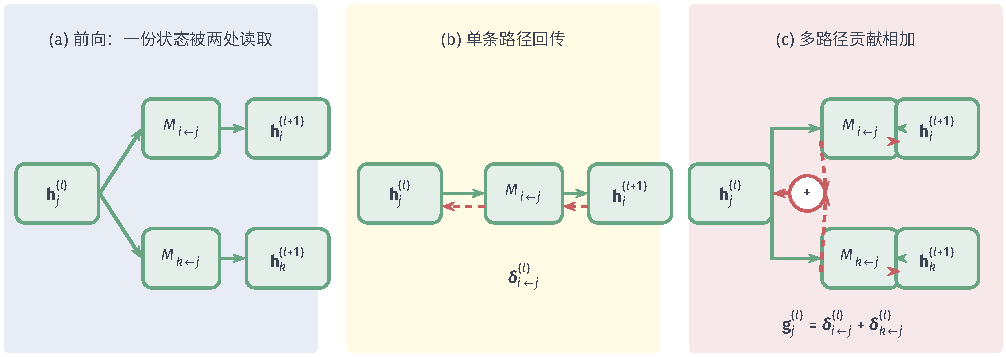
\includegraphics[width=\linewidth]{figures/03-models/02-neural-network-models/tikz/gnn-backpropagation/figure.pdf}
  \caption{一份节点状态的梯度来自多条读取路径。（a）只画前向分叉；（b）单独跟踪一条接收路径的回传；（c）同时回传两条路径，并在$+$处累加为$\bm g_j^{(l)}$。实线表示前向计算，红色虚线表示导数路径。图省略其他邻居的消息、接收节点自身的更新分支和任务输出头；反向依赖由前向读取决定，不要求原图存在反向边。}
  \label{fig:gnn-backpropagation}
\end{figure*}

状态梯度继续传向上一轮，共享参数的梯度则汇集为本次优化器更新的输入。以一层线性消息$\bm{m}_{i\leftarrow j}=\bm{W}\bm{h}_j$为例，$\bm{W}\in\mathbb{R}^{r_l\times m_l}$，接收端回传的消息梯度给发送端贡献$\bm{W}^{\top}\bm{\delta}_{i\leftarrow j}$，并给权重贡献一个外积。因此
\begin{equation}
  \frac{\partial L}{\partial\bm{W}}
    =\sum_{(j\to i)\in E}
      \bm{\delta}_{i\leftarrow j}\bm{h}_j^{\top}\text{。}
  \label{eq:gnn-shared-gradient}
\end{equation}
跨轮共享$\bm{W}$时，还要对轮次求和。节点更新、输入编码及输出头中的共享参数使用同样规则，正则项的导数另加到相应参数。所有贡献计算完毕后才更新参数；边上的梯度不是每个节点各自修改一份独立权重。

\begin{example}[无标签节点怎样得到梯度]
\label{ex:gnn-unlabeled-gradient}
沿用示例~\ref{ex:gnn-two-rounds}的两轮平均，只在节点1设置目标0，取$L=\tfrac12(h_1^{(2)})^2$。此处状态与梯度都是标量，记$g_i^{(l)}=\partial L/\partial h_i^{(l)}$。由$h_1^{(2)}=3/4$，最终轮梯度为$(3/4,0,0)$。节点1的第二轮输出平均了上一轮节点1和2的状态，故
\[
  \bm{g}^{(1)}=(3/8,3/8,0)^{\top},\qquad
  \bm{g}^{(0)}=(5/16,5/16,1/8)^{\top}\text{。}
\]
例如节点3没有标签，却通过节点2影响节点1；它在初始轮收到的梯度为$(3/8)\times(1/3)=1/8$。这里没有可学习的传播参数，例子只核对状态导数。固定输入属性可以具有导数，但不会因此自动成为需要优化的参数。
\end{example}

\subsubsection{训练批次与信息范围}
\label{sec:gnn-training-batches}

\term{全图训练}（full-graph training）在每次前向计算中读取完整训练可见图，再在受监督位置计算损失。单图节点分类可以只抽取一批标签位置，却仍计算全图表示；它与只读取部分结构的训练不同。多个图可以通过块对角邻接矩阵组成一个不连通的大图批次，但读出必须保留各图的归属，不能把不同分子的节点一起求和。

大图上的$L$跳邻域可能迅速膨胀。\term{邻居采样}（neighbor sampling）为本批目标节点逐层选择有限邻居，再在所需计算图上前向和反向。每层最多取$s$个邻居时，未经去重的展开规模可达到$1+s+\cdots+s^L$；采样限制了每步分支数，却没有消除深度影响。均匀采样的均值可无偏估计一个固定邻域向量的平均，但非线性更新后的预测及其梯度通常不是全图结果的无偏估计，归一化和多层抽样还会进一步改变计算。

\term{子图训练}（subgraph training）抽取一部分节点及相应边，在这张子图中完成多轮传播。它便于多个目标共享计算，但截断边界改变了邻域。若希望保留目标节点完整的$L$跳计算，可以把外围节点作为上下文纳入；若只是使用诱导子图，就应说明采用了怎样的近似和归一化。采样误差、边界缺失和标签抽样是不同的变化来源。

数据的可见范围还取决于预测设定。\term{直推学习}（transductive learning）针对训练时已知的一批对象预测未知标签：例如引用图的结构与全文特征可以全部可见，只在部分节点上提供标签。\term{归纳学习}（inductive learning）要求把学到的规则用于此前没有见过的节点或图：训练阶段不能读取这些对象的未来信息。两种设定都可以使用共享消息函数；“参数与节点编号无关”是结构性质，“模型对新对象表现可靠”仍是需要检验的泛化结论。

每次训练更新都应明确可见图、输入特征、监督集合和损失平均方式。对连接预测，还须在编码图中移除待评估的目标边及能直接暴露目标的副本；对动态预测，结构和属性只能来自预测时刻以前。这些限制由任务决定，不能通过只隐藏标签来替代。

\subsubsection{参数更新与收敛条件}
\label{sec:gnn-optimization-convergence}

反向传播给出当前参数下的导数，优化器才决定怎样改变参数。将全部可学习参数记为$\bm{\theta}\in\mathbb{R}^{p}$，固定数据与可见图，记训练损失加正则项为$J(\bm{\theta})$。一次普通梯度更新为
\begin{equation}
  \bm{\theta}^{(t+1)}=\bm{\theta}^{(t)}
    -\eta_t\widehat{\bm{g}}^{(t)}\text{，}
  \label{eq:gnn-parameter-update}
\end{equation}
$t$是优化器更新次数，与传播轮次$l$不同；$\eta_t>0$是学习率。全目标求导时$\widehat{\bm{g}}^{(t)}=\nabla J(\bm{\theta}^{(t)})$，抽批次时则是相应计算得到的梯度估计。每次更新都要在同一份参数下完成前向与反向，清空上一次梯度累积，再对本批贡献求和或按约定平均。

网络的多层复合、消息函数和输出头通常使$J$非凸。因而“训练收敛”需要明确指标：损失趋于稳定、梯度变小、参数趋于某一点和找到全局最小值是不同结论。图上使用共享参数或归一化，都不能单独保证最后一个结论。

一个有条件的结果说明梯度法为什么可能稳定降低目标。假定$J$有下界$J_{\inf}$，且梯度是$\beta$-Lipschitz的，即$\lVert\nabla J(\bm{u})-\nabla J(\bm{v})\rVert_2\leq\beta\lVert\bm{u}-\bm{v}\rVert_2$，其中$\beta>0$。沿连接两参数的线段积分梯度，可得
\[
  J(\bm{u})\leq J(\bm{v})+
  \langle\nabla J(\bm{v}),\bm{u}-\bm{v}\rangle
  +\frac{\beta}{2}\lVert\bm{u}-\bm{v}\rVert_2^2\text{。}
\]
若使用完整梯度与固定学习率$0<\eta\leq1/\beta$，代入式\eqref{eq:gnn-parameter-update}即得到
\begin{equation}
  \begin{aligned}
    J(\bm{\theta}^{(t+1)})
      &\leq J(\bm{\theta}^{(t)})
        -\frac{\eta}{2}\lVert\nabla J(\bm{\theta}^{(t)})\rVert_2^2,\\
    \min_{0\leq t<T}\lVert\nabla J(\bm{\theta}^{(t)})\rVert_2^2
      &\leq\frac{2[J(\bm{\theta}^{(0)})-J_{\inf}]}{\eta T}\text{。}
  \end{aligned}
  \label{eq:gnn-gradient-descent-bound}
\end{equation}
第二行由第一行对$T$次更新求和得到，$T$是优化步数。它保证存在梯度较小的迭代点；在这些假设下完整序列的梯度范数也趋于零，却不保证参数序列一定收敛，更不把驻点变成全局最小值。ReLU及最大聚合具有不可微位置，任意图网络也未必有全局有限的$\beta$，所以不能未经核对便把这段光滑分析套到实际训练上。

抽样梯度还增加了波动。若它在给定参数下无偏、方差有统一上界，并满足相应光滑性及下界条件，递减学习率可以控制梯度噪声。经典条件包括$\sum_t\eta_t=\infty$和$\sum_t\eta_t^2<\infty$，能保证按学习率加权的期望梯度平方范数平均值趋于零，仍不是参数或全局最优解的收敛保证。固定非零学习率通常只能保证平均梯度大小受噪声项控制，单步损失不必持续下降。Bottou等的分析明确区分了这两种情形\scite{bottou2018optimization} 在固定编码图上，均匀抽取标签位置并按目标正确缩放，可以保持完整标签平均损失的无偏梯度；邻居采样经过多层非线性却未必如此。须先确定究竟在优化哪个目标，才能使用相应收敛结论；上述结论也不能自动推广到任意自适应优化器。

实际停止可结合最大步数、在固定评估计算上的训练损失与梯度范数，以及验证指标的早停。传播深度、初始化、度归一化、残差与门控会影响链式Jacobian的尺度，从而影响梯度过小或过大的程度；学习率和优化器也须与该尺度匹配。这些设计改善训练条件的可能性需要检验。固定参数下的状态迭代是否收敛则是另一问题，第~\ref{sec:gnn-state-convergence}节讨论其充分条件；训练目标稳定也不能替代泛化检验。

\section{卷积图神经网络}
\label{sec:gnn-convolutional}

第~\ref{sec:cnn-convolution-definition}节的离散卷积在每个位置使用同一组核系数。一维有限核可写为$y_i=\sum_{r=-K}^{K}w_r x_{i-r}$：位置$i$改变时，系数$w_r$仍对应同一个相对偏移。图也需要共享关系上的计算，却通常没有统一的相对坐标。不同节点的邻居数不同，邻居没有自然次序，也没有一个可在整张图上反复移动的固定窗口。因此，不能直接把图节点编号代入$i-r$；编号的差不表示关系距离。

\term{图卷积}（graph convolution）把规则网格上的共享滤波推广到图信号，即节点上的数值或特征。这个推广有两个互补入口。谱域保留经典卷积定理的形式：先把信号分解成模式，再对各模式的系数乘以滤波响应。空域保留共享局部组合的形式：沿图的邻域，用同一个消息规则计算贡献，再作不依赖邻居次序的聚合。一般图缺少普通平移，因而这里的“卷积”是图上的算子定义，不表示存在一个可以照搬的核翻转与窗口滑动过程。

一个线性图滤波器可以把两种入口联系起来。令$\bm{Q}\in\mathbb{R}^{n\times n}$是给定的局部传播矩阵，非对角非零元只位于相邻节点间；邻接矩阵就是一个选择。对$\bm{H}\in\mathbb{R}^{n\times d_{\mathrm{in}}}$，可定义
\begin{equation}
  \bm{Z}=\sum_{k=0}^{K}\bm{Q}^{k}\bm{H}\bm{W}_k,
  \qquad \bm{W}_k\in\mathbb{R}^{d_{\mathrm{in}}\times d_{\mathrm{out}}}\text{。}
  \label{eq:gnn-polynomial-convolution}
\end{equation}
其中$\bm{Q}^0=\bm{I}_n$，$\bm{Z}\in\mathbb{R}^{n\times d_{\mathrm{out}}}$；$k=0$处理自身，$k\geq1$组织至多$k$跳内经传播到达的信息。$\bm{W}_k$在所有节点共享，并不为每条具体路径另设参数。计算时递推$\bm{H}_0=\bm{H}$、$\bm{H}_k=\bm{Q}\bm{H}_{k-1}$，累加$\bm{H}_k\bm{W}_k$，无需显式形成通常更稠密的$\bm{Q}^k$。非线性激活再作用于$\bm{Z}$，多层这样的计算构成网络。

式\eqref{eq:gnn-polynomial-convolution}如何包含普通卷积，可以在周期的一维有向网格上看清。取移位矩阵$\bm{T}$，满足$(\bm{T}\bm{x})_i=x_{i-1}$，下标按周期返回；则单通道有限核的循环卷积是$\sum_{r=-K}^{K}w_r\bm{T}^{r}\bm{x}$。不同偏移对应重复移位或反向移位。一般图改用邻接或拉普拉斯等关系算子组织传播；无向图上的单个对称算子没有区分左右的标记，不能据此复原任意具有方向差别的网格卷积核。需要方向或关系类型时，应提供相应信息并使用不同关系算子。

共享还必须服从重编号。若$\bm{Q}'=\bm{P}\bm{Q}\bm{P}^{\top}$、$\bm{H}'=\bm{P}\bm{H}$，则$\bm{Z}'=\bm{P}\bm{Z}$，因为$(\bm{P}\bm{Q}\bm{P}^{\top})^k\bm{P}=\bm{P}\bm{Q}^k$。这使局部组合不依赖节点保存次序。但一般消息传递比线性卷积更广：注意力或非线性边消息可以让权重依赖输入，不必对应某个固定的线性频率响应。下面分别从图信号的模式与邻域计算定义具体算子，再比较两者的联系和适用条件。

\subsection{谱域图神经网络}
\label{sec:gnn-spectral}

\subsubsection{图拉普拉斯与图傅里叶变换}
\label{sec:gnn-graph-fourier}

沿用\BookSectionRef{sec:signal-analysis-graph-state-kernels}{第一卷“数学准备”的图谱变换与局部传播小节}，
在对称非负邻接矩阵上使用图拉普拉斯及图傅里叶坐标。
低频表示相连节点上的归一化信号变化较小；本节要学习的是各频率如何影响输出，
而不是重新建立图谱理论。

记$d_i=\sum_j\bm A_{i,j}$为节点度，$\bm D=\operatorname{diag}(d_1,\ldots,d_n)$为度矩阵。
节点度差异较大时，常用\term{对称归一化拉普拉斯}（symmetric normalized Laplacian）。
本节为简化推导，假定所有节点$d_i>0$，令
\begin{equation}
  \bm{L}=\bm{I}_n-\bm{D}^{-1/2}\bm{A}\bm{D}^{-1/2}
    =\bm{U}\bm{\Lambda}\bm{U}^{\top}\text{。}
  \label{eq:gnn-laplacian-spectrum}
\end{equation}
$\bm{U}\in\mathbb{R}^{n\times n}$的列$\bm{u}_k$是正交特征向量，$\bm{\Lambda}$的对角元素$\lambda_k\in[0,2]$按升序排列。归一化后的能量比较$x_i/\sqrt{d_i}$与$x_j/\sqrt{d_j}$，因此零频模式在每个连通分量内与$\sqrt{d_i}$成比例，未必是常量；不同分量可以具有不同的比例系数。图连通时，零特征空间才只有这一个方向。存在孤立节点时须另规定归一化约定，或加自环后再定义相应算子。

在卷一的图傅里叶坐标$\widehat{\bm x}=\bm U^\top\bm x$中，
让频率响应$g_{\bm\theta}(\lambda)$随训练参数改变，得到可学习的谱滤波：
\begin{equation}
  \bm{y}=\bm{U}g_{\bm{\theta}}(\bm{\Lambda})\bm{U}^{\top}\bm{x}
    =g_{\bm{\theta}}(\bm{L})\bm{x}\text{。}
  \label{eq:gnn-spectral-filter}
\end{equation}
图~\ref{fig:gnn-spectral-filter}显示这三步。谱域图卷积借用了经典卷积在傅里叶域逐频率相乘的形式；一般图上的这一命名不保证它具有普通空间平移的含义。

\begin{figure*}[htb]
  \centering
  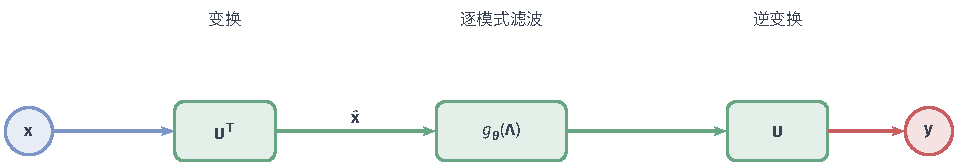
\includegraphics[width=\linewidth]{figures/03-models/02-neural-network-models/tikz/gnn-spectral-filter/figure.pdf}
  \caption{谱滤波的计算路径。节点信号$\bm{x}$经$\bm{U}^{\top}$分解为图傅里叶系数，每个模式由$g_{\bm{\theta}}(\lambda_k)$调整，再经$\bm{U}$还原为节点信号。左、右两端使用同一张图和同一节点顺序；中间向量的下标表示频率模式。}
  \label{fig:gnn-spectral-filter}
\end{figure*}

\begin{example}[三节点路径上的低频模式]
\label{ex:gnn-low-frequency}
沿用路径$1-2-3$，此处不加自环，度为$(1,2,1)$。归一化拉普拉斯的特征值为$0,1,2$，可取
\[
  \bm{u}_1=\tfrac12(1,\sqrt2,1)^{\top},\quad
  \bm{u}_2=\tfrac{1}{\sqrt2}(1,0,-1)^{\top},\quad
  \bm{u}_3=\tfrac12(1,-\sqrt2,1)^{\top}\text{。}
\]
输入$\bm{x}=(1,0,2)^{\top}$的三个系数为$3/2,-1/\sqrt2,3/2$。若只保留零频模式，输出为$(3/4,3\sqrt2/4,3/4)^{\top}$。中间节点的数值较大，恰是度归一化后的平滑，而不是普通算术平均。
\end{example}

\subsubsection{Spectral CNN：直接学习频率响应}
\label{sec:gnn-spectral-cnn}

Bruna等的Spectral CNN把谱滤波放入多通道网络。对输入通道$a$与输出通道$b$，可以学习一个对角滤波器$\bm{\Theta}_{a,b}$，用$\bm{U}\bm{\Theta}_{a,b}\bm{U}^{\top}$变换对应信号，再累加通道并使用非线性。完整谱上的自由响应需要每通道对$n$个参数；原工作还用少量样条系数插值得到平滑响应，减少参数自由度\scite{bruna2014spectral}

固定图与傅里叶基时，前向计算是矩阵乘法，滤波参数可按链式法则求导。例如单通道$\bm{y}=\bm{U}\operatorname{diag}(\bm{\theta})\widehat{\bm{x}}$，上游梯度为$\bm{v}=\partial L/\partial\bm{y}$，则$\partial L/\partial\theta_k=(\bm{U}^{\top}\bm{v})_k\widehat x_k$。通道与样本之间共享参数时，对相应贡献求和即可。

直接使用稠密$\bm{U}$需要$O(n^2)$的单信号变换和存储，完整稠密特征分解的常规代价为$O(n^3)$。只保留部分特征向量可以改变代价，但也限制了可用模式。自由频率响应还可能对应全图稠密算子，不能仅凭“卷积”就认定它具有有限跳数的局部性。

对新图，特征值与特征向量都会变化，按旧图谱索引学习的自由系数没有自然的一一对应。特征向量的符号在$\bm{U}\bm{\Theta}\bm{U}^{\top}$中相消，但重特征值对应的子空间还可以旋转；若该子空间内使用不同自由系数，算子就依赖具体基的选择。由同一个标量函数$g(\lambda)$定义响应，能够消除这种基选择歧义；跨图迁移的预测效果仍需另行验证。

\subsubsection{ChebNet：用多项式实现局部滤波}
\label{sec:gnn-chebnet}

若滤波器能够直接写成$\bm{L}$的多项式，就可以绕开显式傅里叶基。ChebNet用\term{切比雪夫多项式}（Chebyshev polynomial）参数化响应。设$\lambda_*>0$是拉普拉斯谱的上界，令$\widetilde{\bm{L}}=2\bm{L}/\lambda_*-\bm{I}_n$，把谱放到$[-1,1]$；归一化拉普拉斯可取$\lambda_*=2$。约定$K$为最高次数，则
\begin{equation}
  g_{\bm{\theta}}(\bm{L})\bm{x}
    =\sum_{k=0}^{K}\theta_k T_k(\widetilde{\bm{L}})\bm{x}\text{，}
  \label{eq:gnn-chebyshev-filter}
\end{equation}
其中$T_0(z)=1$、$T_1(z)=z$、$T_k(z)=2zT_{k-1}(z)-T_{k-2}(z)$。有些文献用$K$表示项数，此时最高次数为$K-1$，阅读时须核对约定\scite{defferrard2016chebnet}

令$\bm{z}_k=T_k(\widetilde{\bm{L}})\bm{x}$，即可用$\bm{z}_0=\bm{x}$、$\bm{z}_1=\widetilde{\bm{L}}\bm{x}$以及$\bm{z}_k=2\widetilde{\bm{L}}\bm{z}_{k-1}-\bm{z}_{k-2}$递推。整个过程只需要稀疏矩阵乘向量；单通道的$K\geq1$阶计算量为$O(K(n+e))$，无需构造$\bm{U}$。反向传播也经过这些稀疏乘法，系数梯度为$\bm{v}^{\top}\bm{z}_k$。

多项式为何局部，可以从矩阵乘法看出。$\bm{L}$的非对角非零元只连接相邻节点，一次相乘至多走一条边；$\bm{L}^k$至多连接$k$跳以内。故式\eqref{eq:gnn-chebyshev-filter}在一层中读取至多$K$跳邻域。多通道形式为$\bm{Y}=\sum_{k=0}^{K}T_k(\widetilde{\bm{L}})\bm{X}\bm{\Theta}_k$，$\bm{\Theta}_k\in\mathbb{R}^{d_{\mathrm{in}}\times d_{\mathrm{out}}}$，参数量为$(K+1)d_{\mathrm{in}}d_{\mathrm{out}}$，不随$n$增加。

这些系数描述同一个多项式，所以可以在另一张图上重新构造拉普拉斯并使用它们，无需对齐特征向量。相同计算规则能够运行在新图上，并不保证新图具有相同的频率分布或任务关系。若使用的谱上界过小，使缩放后的特征值落到$[-1,1]$以外，高次多项式还可能迅速放大误差。

\subsection{空域图神经网络}
\label{sec:gnn-spatial}

空域方法直接回答节点怎样读取邻居。下面四种模型分别突出固定归一化、采样与分开组合、内容相关加权，以及邻域多重集合的区分能力。它们共享输出与反向传播的基础，主要差别落在聚合和更新上。

\subsubsection{GCN：归一化的邻域传播}
\label{sec:gnn-gcn}

\term{图卷积网络}（graph convolutional network, GCN）在本节特指Kipf与Welling提出的层形式。加入自环$\widetilde{\bm{A}}=\bm{A}+\bm{I}_n$，令$\widetilde d_i=\sum_j\widetilde{\bm{A}}_{i,j}$，定义传播矩阵
\begin{equation}
  \bm{S}=\widetilde{\bm{D}}^{-1/2}\widetilde{\bm{A}}\widetilde{\bm{D}}^{-1/2},
  \qquad
  \bm{H}^{(l+1)}=\sigma\!\left(\bm{S}\bm{H}^{(l)}\bm{W}^{(l)}\right)\text{。}
  \label{eq:gnn-gcn-layer}
\end{equation}
$\bm{H}^{(l)}\in\mathbb{R}^{n\times m_l}$按行存放状态，$\bm{H}^{(0)}=\bm{X}$；$\bm{W}^{(l)}\in\mathbb{R}^{m_l\times m_{l+1}}$变换特征通道，$\sigma$逐坐标作用。采用行存放的矩阵形式时，节点列向量的变换对应$(\bm{W}^{(l)})^{\top}\bm{h}_i^{(l)}$。原始层式省略偏置，增加共享偏置不会改变置换等变性。

从节点$j$到$i$的消息系数为$\widetilde{\bm{A}}_{i,j}/\sqrt{\widetilde d_i\widetilde d_j}$，同时计入边权以及接收端与发送端的度。边权为1时，才简化为$1/\sqrt{\widetilde d_i\widetilde d_j}$。它不是一般意义上的算术平均：$\bm{S}$的行和未必等于1。沿用三节点无权路径与输入$(1,0,2)^{\top}$，取单位特征变换和恒等激活，得到
\begin{equation}
  \bm{S}=\begin{pmatrix}
    1/2&1/\sqrt6&0\\
    1/\sqrt6&1/3&1/\sqrt6\\
    0&1/\sqrt6&1/2
  \end{pmatrix},\qquad
  \bm{S}\bm{x}=\begin{pmatrix}1/2\\3/\sqrt6\\1\end{pmatrix}\text{。}
  \label{eq:gnn-gcn-example}
\end{equation}
这一结果与示例~\ref{ex:gnn-two-rounds}的平均不同，差别来自归一化规则。

它与谱域方法的联系可以直接推导。对不加自环的归一化拉普拉斯，ChebNet取$K=1$及$\lambda_*=2$时，$\widetilde{\bm{L}}=-\bm{D}^{-1/2}\bm{A}\bm{D}^{-1/2}$。再约束$\theta_0=-\theta_1=\theta$，得到$\theta(\bm{I}_n+\bm{D}^{-1/2}\bm{A}\bm{D}^{-1/2})\bm{x}$。GCN进一步以加自环后重新计算度的$\bm{S}$替换括号内算子，限制反复传播的尺度。这一步是算子设计，不是二者恒等相等；原论文称其为重新归一化技巧\scite{kipf2017gcn}

固定结构时，GCN的梯度也可写清。记$\bm{Z}=\bm{S}\bm{H}\bm{W}$，$\bm{\Delta}=\partial L/\partial\bm{Z}$，则
\begin{equation}
  \frac{\partial L}{\partial\bm{W}}=(\bm{S}\bm{H})^{\top}\bm{\Delta},\qquad
  \frac{\partial L}{\partial\bm{H}}=\bm{S}^{\top}\bm{\Delta}\bm{W}^{\top}\text{。}
  \label{eq:gnn-gcn-backprop}
\end{equation}
激活的导数已并入$\bm{\Delta}$。不学习邻接关系时，$\bm{S}$作为给定算子；学习边权或建图规则时，才需进一步计算结构相关梯度。

标准GCN直接混合相邻节点的变换特征。相邻对象与预测目标相关时，这种共享聚合可以提供有用信息；相邻节点常具有不同标签或关系语义时，混合也可能损失区分所需的特征。模型仍可在新图上使用共享权重，归纳能力不由“GCN”或原论文的直推实验设定单独决定。

\subsubsection{GraphSAGE：采样并学习邻域组合}
\label{sec:gnn-graphsage}

在很大的图上，为一批目标节点计算全部邻域代价高；新节点到达后，也希望直接用属性及邻域产生表示。GraphSAGE把采样与聚合纳入这一过程。以平均聚合为例，从$N(i)$中取$S_i^{(l)}$，令
\begin{equation}
  \begin{aligned}
    \bm{u}_i^{(l)}&=\frac{1}{|S_i^{(l)}|}\sum_{j\in S_i^{(l)}}\bm{h}_j^{(l)},\\
    \bm{h}_i^{(l+1)}&=\sigma\!\left(
      \bm{W}^{(l)}[\bm{h}_i^{(l)};\bm{u}_i^{(l)}]+\bm{b}^{(l)}\right)\text{。}
  \end{aligned}
  \label{eq:gnn-graphsage}
\end{equation}
分号表示向量拼接，此处$\bm{W}^{(l)}\in\mathbb{R}^{m_{l+1}\times2m_l}$。自身和邻居先分开，再由不同的权重块组合；原算法还可对输出作$\ell_2$归一化，零向量需要单独处理\scite{hamilton2017graphsage}

聚合器也可对邻居先作共享前馈变换，再取逐坐标最大值。平均保留总体水平，最大池化突出某种响应是否出现。原论文还试验了对随机邻居顺序使用LSTM的聚合器；LSTM本身依赖次序，随机打乱不能使一次确定性输出严格置换不变。需要严格对称性时，应选用对称聚合，或明确说明采用了怎样的对称化。

训练时采样所需邻域，计算节点或关系任务的损失，联合更新聚合器、组合矩阵及输出头。预测新节点时沿相同规则读取可用特征与邻域，不必为它单独学习一个节点编号嵌入。若新节点没有特征或可用邻居，模型仍受信息不足限制；若只把节点编号作为输入，所谓归纳流程也失去了可迁移的属性基础。

\subsubsection{GAT：根据内容调整邻居权重}
\label{sec:gnn-gat}

固定度归一化没有区分“邻居与当前任务是否相关”。\term{图注意力网络}（graph attention network, GAT）用节点特征计算邻居权重，再在图约束的可见范围内加权聚合。对一个注意力头，令$\bm{z}_i=\bm{W}\bm{h}_i$，其中$\bm{W}\in\mathbb{R}^{m'\times m}$，则
\begin{equation}
  \begin{aligned}
    e_{i,j}&=\operatorname{LeakyReLU}
      \!\left(\bm{a}^{\top}[\bm{z}_i;\bm{z}_j]\right),\\
    \alpha_{i,j}&=\frac{\exp(e_{i,j})}
      {\sum_{k\in N(i)\cup\{i\}}\exp(e_{i,k})},\\
    \bm{h}'_i&=\sigma\!\left(\sum_{j\in N(i)\cup\{i\}}
      \alpha_{i,j}\bm{z}_j\right)\text{。}
  \end{aligned}
  \label{eq:gnn-gat}
\end{equation}
$\bm{a}\in\mathbb{R}^{2m'}$是共享评分参数；$e_{i,j}$是标量得分，与本章的边数$e$不同。Softmax只在节点$i$的可见邻域内归一化，所有节点使用同一评分函数，所以邻居重排只重排对应权重\scite{velickovic2018gat}

多头注意力分别学习变换和评分，在隐藏层拼接结果，或在输出层取平均。训练时梯度同时通过值向量和权重；若把权重当作常量，就漏掉了评分函数对损失的影响。固定每头宽度时，增加头数还会增加总宽度和参数量，比较必须注明宽度预算。

与前章的循环注意力一样，GAT把“计算权重”和“读取信息”分开；区别是可见位置由图的邻接关系约束。原始GAT的评分使用线性拼接，若将$\bm{a}$拆成两部分，得分是单调激活作用于一个接收端项与一个发送端项之和。因此，在固定候选邻居特征下，邻居排序不能仅靠改变接收端特征任意翻转。内容相关权重并不意味着原始评分能够表达所有成对选择关系。

注意力可以重新分配已有邻居的影响，却不能一轮读取不在可见范围内的节点。权重归一化也不能保证这些权重等同于可靠的解释或因果贡献；输出仍由表示、评分、后续变换和训练共同决定。

\subsubsection{GIN：保留邻域多重集合的差别}
\label{sec:gnn-gin}

聚合不仅影响尺度，还决定哪些输入差异会在计算中消失。例如邻域$\{\!\{1,1\}\!\}$与$\{\!\{1,1,1\}\!\}$具有相同平均和最大值，但个数不同。另一个例子$\{\!\{0,2\}\!\}$与$\{\!\{1,1\}\!\}$连原始数值的和也相同；求和需要配合合适的特征映射，才能保留更多差别。图~\ref{fig:gnn-aggregation}展示第一种信息损失。

\begin{figure*}[htb]
  \centering
  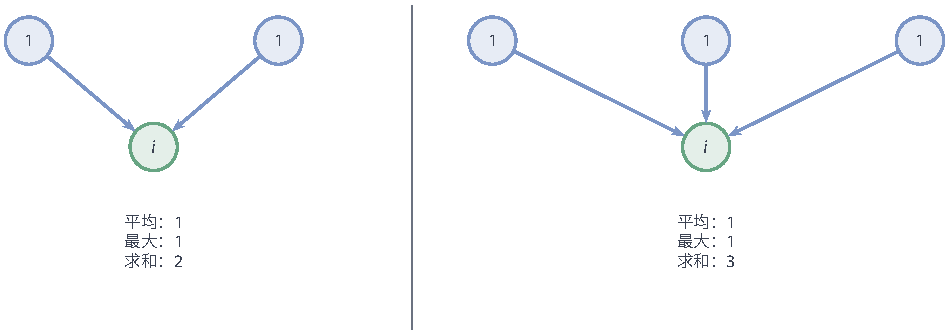
\includegraphics[width=\linewidth]{figures/03-models/02-neural-network-models/tikz/gnn-aggregation/figure.pdf}
  \caption{聚合如何保留或丢掉重复次数。两个邻域分别含两个和三个数值为1的邻居。平均与最大值都产生1，求和分别产生2和3。图只比较固定标量消息；求和本身也不能区分所有不同多重集合，还需要合适的特征映射。}
  \label{fig:gnn-aggregation}
\end{figure*}

\term{图同构网络}（graph isomorphism network, GIN）使用求和聚合与前馈更新：
\begin{equation}
  \bm{h}_i^{(l+1)}=\operatorname{MLP}^{(l)}\!\left(
    (1+\epsilon^{(l)})\bm{h}_i^{(l)}
      +\sum_{j\in N(i)}\bm{h}_j^{(l)}\right)\text{，}
  \label{eq:gnn-gin}
\end{equation}
$\epsilon^{(l)}$可以固定或学习，用于区分中心节点与邻居的贡献。参数通过任务损失反向传播；整图读出还可拼接各层节点求和，保留不同传播范围的信息\scite{xu2019gin}

比较两张图时，若存在保持连接关系及给定属性的节点重编号，使两图相互对应，就称它们\term{同构}（isomorphic）。图同构网络的名称并不表示它能判定任意两图是否同构。衡量其区分能力的一种参照是\term{一维Weisfeiler--Leman检验}（1-dimensional Weisfeiler--Leman test, 1-WL）：从与节点属性一致的初始标记出发，反复用“节点旧标记及邻居标记的多重集合”产生新标记。所比较的图必须使用同一套无冲突标记规则，相同的输入组合得到相同标记，不同组合得到不同标记。每轮比较两图全部节点标记组成的多重集合；只要有一轮不同，就可判为非同构，始终相同则不能证明同构。

对于只使用节点状态、对称邻域聚合且不引入额外区分信息的消息传递网络，1-WL无法区分的图也不能靠这些更新与节点多重集合读出区分：同标记节点具有同样的邻域标记多重集合，共享计算遂逐轮产生同样的状态。

在可数特征域、邻域大小有界，以及聚合、更新和读出满足相应单射性条件时，求和特征映射可以达到1-WL的区分能力。\term{单射}（injective）表示不同输入不会被映成同一个结果；有限宽度网络与训练算法并不自动满足该条件，也不能把这一理论直接推广为对所有连续特征无条件成立的保证。

1-WL本身也有边界。六节点环与两个互不连接的三角形都具有六个节点，每个节点度为2。若初始节点特征全部相同，这两张图上的节点在每轮都会收到两个相同状态，任何上述消息传递加节点多重集合读出都无法区分它们。增加传播轮数不能改变这一对称性；需要子结构信息、更高阶状态或其他符合任务要求的输入。能区分更多图是一种表达性质，也不等于训练样本上的泛化一定更好。

\subsection{谱域与空域的联系、区别及选择}
\label{sec:gnn-spectral-spatial-comparison}

谱域与空域的区别主要在于怎样规定算子，而不是计算一定发生在哪一类存储空间。谱域用$g_{\bm{\theta}}(\lambda)$规定不同变化模式的响应，空域用邻居的选择、消息和聚合规定局部组合。若$g_{\bm{\theta}}$是多项式，$\bm{U}g_{\bm{\theta}}(\bm{\Lambda})\bm{U}^{\top}$等于同一多项式作用于$\bm{L}$，便可完全通过节点域稀疏传播计算。ChebNet由谱域设计、按邻域递推实现，GCN也保留了谱域推导。因此，把谱域等同于特征分解、把空域等同于没有频率含义，会把这部分交集漏掉。

表~\ref{tab:gnn-spectral-spatial}将显式谱实现与多项式实现分开。比较计算量时固定一张稀疏图与单通道线性传播，不计特征通道变换、消息网络及初次特征分解的代价；任意空域消息网络的成本还取决于其具体函数。
\begin{table*}[htb]
  \centering
  \small
  \begin{tabularx}{\linewidth}{@{}p{17mm}XXX@{}}
    \toprule
    比较方面 & 显式谱基滤波 & 多项式谱滤波 & 局部空域聚合\\
    \midrule
    算子定义 & 在图傅里叶模式上规定响应 & 用低阶多项式参数化响应 & 用邻居消息、权重及更新规定组合\\
    实际计算 & $\bm{U}^{\top}$、对角滤波、$\bm{U}$ & 拉普拉斯的稀疏乘法递推 & 沿可见边计算，再按节点聚合\\
    局部范围 & 自由响应通常涉及全图 & $K$次多项式至多读取$K$跳 & 一轮通常读取一跳；可另加长程边\\
    传播成本 & 稠密基下$O(n^2)$ & $O(K(n+e))$ & 一跳简单聚合为$O(n+e)$\\
    跨图使用 & 按旧谱索引的自由参数缺少自然对应 & 共享多项式系数，在新图重建算子 & 共享消息规则，在新图读取邻域\\
    \bottomrule
  \end{tabularx}
  \caption{谱域与空域图卷积的比较。显式谱基滤波表示直接使用完整图傅里叶基的实现；多项式谱滤波同时具有有限邻域解释。跨图使用一行只说明计算规则能否复用，不能据此保证新图上的预测效果。}
  \label{tab:gnn-spectral-spatial}
\end{table*}

在大图、多个大小不同的图或不断变化的图上，直接依赖完整$\bm{U}$有几项实际困难。特征分解与稠密变换占用时间和存储，图结构改变后还需处理新的谱；按某张图谱索引学习的系数无法直接对应另一张图的模式。一般自由响应又不是严格局部的，一批目标节点可能依赖大量其他节点，难以只取少量邻居完成同一计算。这些条件解释了为何直接使用完整特征基的早期实现较少成为大规模局部模型的计算方式。

沿边的空域计算容易与邻居采样及小批次结合，也便于让消息读取边类型、方向和接收端内容。复杂度在稀疏图与固定宽度下可随边数增长，参数不必随节点数增加。这些是选择空域组织的具体理由，但局部可执行并不保证容易优化，也不自动解决有限传播距离、过平滑或过压缩。多项式谱滤波同样可以绕开特征分解并共享参数；不能把早期显式谱实现的全部困难归给它。

完整谱基、多项式滤波和空域聚合提供了不同的计算取舍，选择时应回到所需关系。若关心图信号哪些频率应保留或抑制，谱响应提供了直接的设计和分析对象；若需要不同边类型、内容相关交互或采样邻域，空域消息规则更便于表达这些计算。固定线性滤波、有限邻域与跨图复用可以同时成立；输入相关的非线性消息则未必是单个固定谱滤波器。比较两类网络时，应同时写清算子定义、实际实现、可见范围和数据条件。

谱滤波的后续研究继续改进参数化与计算方式。2022年的ChebNetII通过切比雪夫插值组织可学习的谱响应，改进原有滤波器的参数化\scite{he2022chebnetii} 2026年的L2G-NET研究图傅里叶变换的结构化分解，用子图谱表示及其组合处理局部与全局信息，针对完整谱变换的成本和局部性提出新的计算方式\scite{fernandez2026l2gnet} 这些工作进一步探索了频率响应、局部传播和全局交互之间的联系，各自的收益需要结合任务与数据检验。

\section{循环图神经网络}
\label{sec:gnn-recurrent}

前面的网络可以为每层学习不同的变换。若希望同一套关系推理反复执行，就可以跨传播轮次共享参数。本节始终固定输入图；传播轮次表示算法内部更新次数，现实时间变化另在第~\ref{sec:gnn-dynamic}节处理。

\subsection{网络结构}
\label{sec:gnn-recurrent-structure}

\term{循环图神经网络}（recurrent graph neural network）在同一图上反复更新节点隐状态。将全部状态按节点堆成列向量$\bm{h}^{(t)}\in\mathbb{R}^{nm}$，令参数向量为$\bm{\theta}\in\mathbb{R}^{p}$，可写为
\begin{equation}
  \bm{h}^{(t+1)}=F_{\bm{\theta}}(\bm{h}^{(t)};\mathcal{G},\bm{X}),
  \qquad \widehat{\bm{y}}=g_{\bm{\theta}}(\bm{h}^{(T)})\text{。}
  \label{eq:gnn-recurrent-update}
\end{equation}
$F_{\bm{\theta}}$内部仍包含共享消息、聚合与节点更新；分号后的图与属性在各轮固定。图~\ref{fig:gnn-recurrent}显示同一规则的多次调用，每次调用的状态值不同。跨轮共享还要求相应状态维度兼容。

\begin{figure*}[htb]
  \centering
  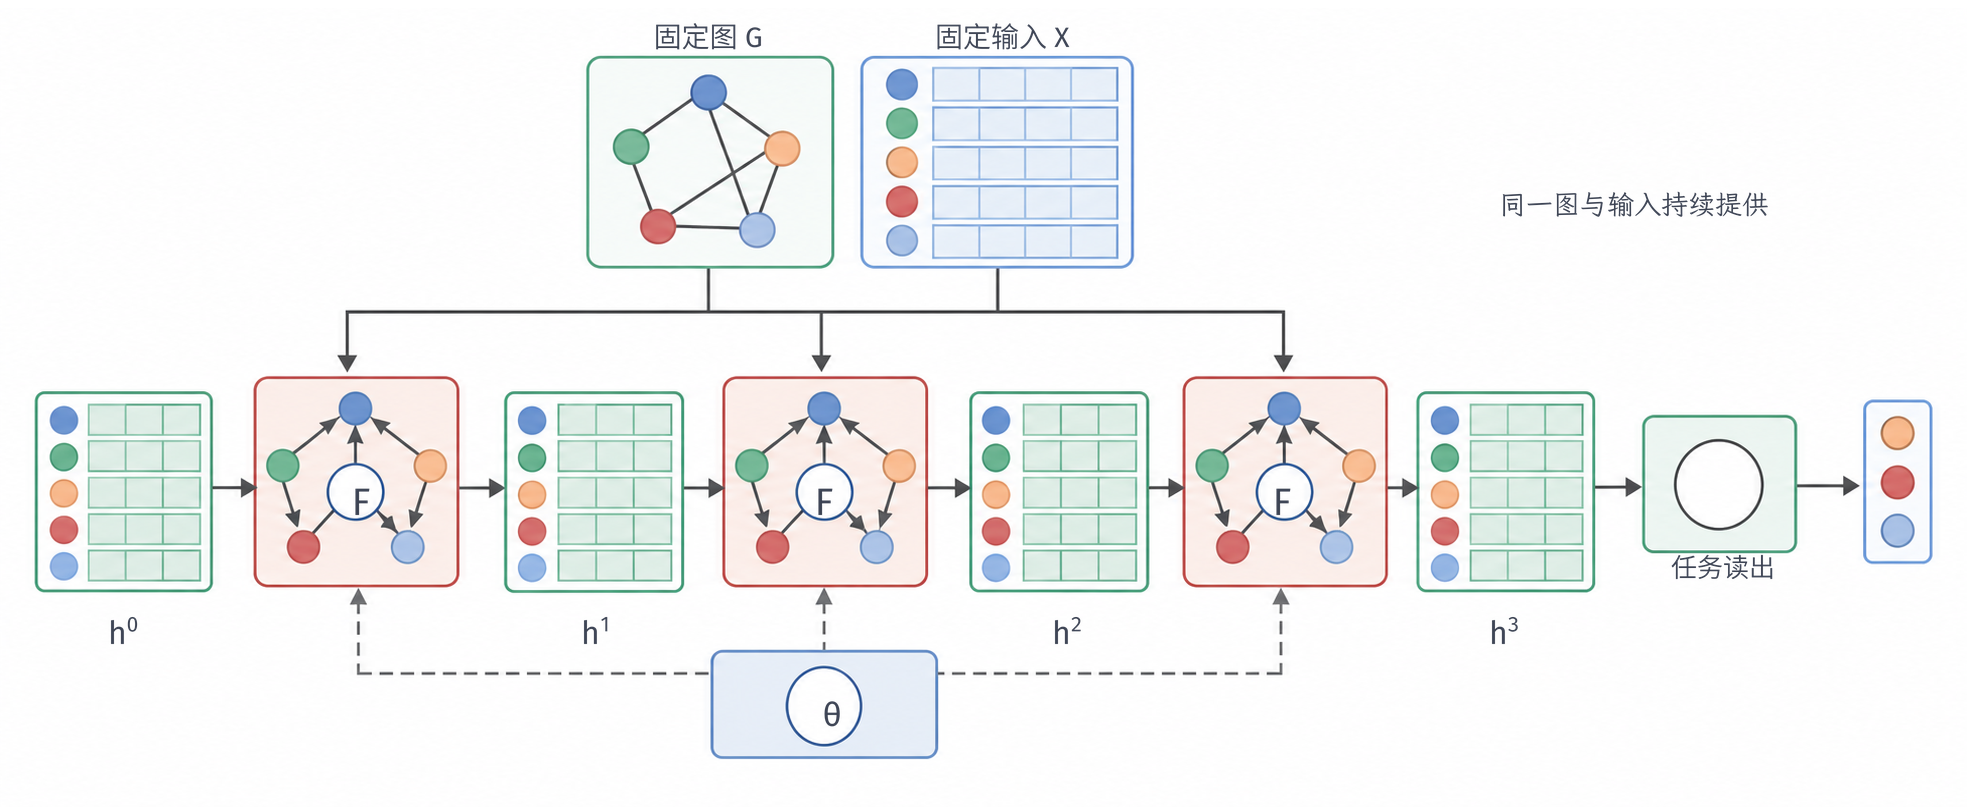
\includegraphics[width=\linewidth]{figures/03-models/02-neural-network-models/generated/gnn-recurrent/figure.png}
  \caption{固定图上的循环更新。左侧表示邻接关系，右侧展开三轮共享更新$F_{\bm{\theta}}$，每个状态向量包含整张图的节点状态。路径提供固定的图与输入特征，路径传递状态，路径读出任务结果。轮次是内部计算步，不表示图已经发生三个时间点的变化。}
  \label{fig:gnn-recurrent}
\end{figure*}

共享参数减少了随轮数增长的参数自由度，却没有减少必须执行的轮数。它也没有把多轮传播变成普通图上的最短路或逻辑推理算法；实际保留与传播什么信息仍由状态更新和监督决定。有限轮次模型与迭代至稳定的模型分别定义不同的输出。

\subsection{典型模型}
\label{sec:gnn-recurrent-models}

\subsubsection{以不动点为目标的图网络}
\label{sec:gnn-fixed-point-model}

早期GNN把目标状态定义为\term{不动点}（fixed point）：再次使用更新函数后仍不改变的状态，即$\bm{h}^*=F_{\bm{\theta}}(\bm{h}^*;\mathcal{G},\bm{X})$。它通过邻居状态迭代计算这一表示，再读取节点或图输出。为保证状态可确定，模型约束更新对状态具有收缩性；第~\ref{sec:gnn-propagation-theory}节将给出条件及误差界。

这类模型的参数既影响输出映射，也影响不动点的位置。有限精度计算通常在相邻两轮差小于容差时停止，并设置最大轮数。若未达到停止条件就触及上限，得到的是当前近似状态；不能把“程序停止了”当作“已经收敛到所定义的不动点”。收缩约束也限制了允许的状态动态，并非所有更新函数都满足它。

\subsubsection{GGNN：固定轮次的门控传播}
\label{sec:gnn-ggnn}

如果任务只需要执行有限步，可以直接学习这些步骤的结果。\term{门控图神经网络}（gated graph neural network, GGNN）在聚合后用GRU式更新保留或写入状态。令$r(i,j)$表示边的类型与方向，邻域输入为
\begin{equation}
  \bm{a}_i^{(t)}=\sum_{j\in N(i)}\bm{W}_{r(i,j)}\bm{h}_j^{(t-1)}+\bm{b},
  \qquad
  \bm{h}_i^{(t)}=\operatorname{GRU}(\bm{h}_i^{(t-1)},\bm{a}_i^{(t)})\text{。}
  \label{eq:gnn-ggnn}
\end{equation}
这里$\bm{a}_i^{(t)}$是聚合输入向量，与边属性$\bm{a}_{i,j}$通过索引形式区分。原模型分别处理入边与出边并组合相应消息；式\eqref{eq:gnn-ggnn}写出一个统一的关系聚合形式，方向也可编码为不同类型\scite{li2016ggnn}

GRU的门机制沿用第~\ref{sec:rnn-gru}节。若把更新门解释为写入比例，状态可写为$\bm{h}_i^{(t)}=(\bm{1}-\bm{z}_i^{(t)})\odot\bm{h}_i^{(t-1)}+\bm{z}_i^{(t)}\odot\widetilde{\bm{h}}_i^{(t)}$；候选状态同时依赖聚合输入与经重置门处理的旧状态。门为节点提供选择性保留路径，远处证据则仍须沿边经过足够轮次。

GGNN用预先设定的$T$轮展开计算并训练，不要求状态在$T$轮达到不动点。它避免了为收敛强加同一类收缩约束，但也失去了由该约束直接得到的唯一稳定状态保证。训练时的轮次是模型设置；在预测时任意增加轮次，可能改变行为，不能默认等同于“推理更充分”。

\subsection{参数学习}
\label{sec:gnn-recurrent-learning}

有限展开的梯度与随时间反向传播具有相同结构。设局部状态Jacobian矩阵$\bm{J}^{(t)}=\partial\bm{h}^{(t+1)}/\partial\bm{h}^{(t)}$，$\bm{\delta}^{(t)}$为第$t$轮状态的总梯度。若损失只读取末状态，则$\bm{\delta}^{(t)}=(\bm{J}^{(t)})^{\top}\bm{\delta}^{(t+1)}$；中间轮存在直接监督时，另加对应梯度。共享更新参数的梯度为
\begin{equation}
  \nabla_{\bm{\theta}}L
    =\left.\nabla_{\bm{\theta}}L\right|_{\mathrm{direct}}
      +\sum_{t=0}^{T-1}(\bm{B}^{(t)})^{\top}\bm{\delta}^{(t+1)}\text{，}
  \label{eq:gnn-recurrent-gradient}
\end{equation}
其中$\bm{B}^{(t)}=\partial F_{\bm{\theta}}(\bm{h}^{(t)};\mathcal{G},\bm{X})/\partial\bm{\theta}$固定当前输入状态求偏导。直接项包含读出参数等依赖；初态若依赖参数，还需计入初态梯度。截断展开会遗漏更早的间接贡献，降低存储与计算的同时改变所用梯度。

不动点模型还可用\term{隐式微分}（implicit differentiation）：对定义状态的方程求导，而不保存全部前向迭代。假设更新在不动点附近可微，令$\bm{J}_*=\partial F/\partial\bm{h}$、$\bm{B}_*=\partial F/\partial\bm{\theta}$在$\bm{h}^*$处取值。若$\bm{I}-\bm{J}_*$可逆，则
\begin{equation}
  (\bm{I}-\bm{J}_*)\frac{\partial\bm{h}^*}{\partial\bm{\theta}}
    =\bm{B}_*\text{。}
  \label{eq:gnn-implicit-state-gradient}
\end{equation}
这个等式来自对$\bm{h}^*=F_{\bm{\theta}}(\bm{h}^*)$两侧求导，并把状态导数项移到左侧。

实际需要的是标量损失的梯度。记$\bm{v}=\partial L/\partial\bm{h}^*$为列向量，解线性方程
\begin{equation}
  (\bm{I}-\bm{J}_*^{\top})\bm{u}=\bm{v},\qquad
  \nabla_{\bm{\theta}}L
    =\left.\nabla_{\bm{\theta}}L\right|_{\mathrm{direct}}+\bm{B}_*^{\top}\bm{u}\text{。}
  \label{eq:gnn-implicit-loss-gradient}
\end{equation}
无需显式求逆。若相应范数下$\lVert\bm{J}_*\rVert<1$，可用$\bm{u}^{(k+1)}=\bm{v}+\bm{J}_*^{\top}\bm{u}^{(k)}$迭代；Jacobian转置与向量的乘积由自动微分计算。前向状态与后向线性求解都有容差，两者都会影响最终梯度的精度。

对只迭代到近似状态的模型，有限展开给出实际执行步骤的梯度，隐式方法近似理想不动点目标的梯度，二者在尚未充分收敛时未必相同。停止条件、最大轮数和状态收缩速度因而既影响前向代价，也影响参数学习。

\section{图神经网络的扩展}
\label{sec:gnn-extensions}

普通图上的一套聚合规则把每条边都当成成对的信息通路。现实关系还可能具有不同语义，随时间变化，涉及多个参与者，或依赖空间位置。扩展模型需要保留这些输入差异，并把它们放到相应的消息、状态和对称性约束中。

\subsection{多关系与异构图}
\label{sec:gnn-relational}

“论文引用论文”与“作者撰写论文”不是同一种关系，把它们混在同一平均中会丢掉关系含义。\term{多关系图}（multi-relational graph）允许边具有不同关系类型；\term{异构图}（heterogeneous graph）还允许不同节点类型具有不同的属性和角色。两者可以同时存在，但边类型多并不必然意味着节点类型也不同。

设关系类型集合为$R$，$N_r(i)$是通过类型$r$向$i$发送消息的邻居。\term{关系图卷积网络}（relational graph convolutional network, R-GCN）为不同关系使用不同变换：
\begin{equation}
  \bm{h}_i^{(l+1)}=\sigma\!\left(
    \bm{W}_0^{(l)}\bm{h}_i^{(l)}+
    \sum_{r\in R}\sum_{j\in N_r(i)}
      \frac{1}{c_{i,r}}\bm{W}_r^{(l)}\bm{h}_j^{(l)}\right)\text{。}
  \label{eq:gnn-rgcn}
\end{equation}
$c_{i,r}>0$是归一化系数，可在非空邻域取$|N_r(i)|$；空邻域的求和直接为零。$\bm{W}_0^{(l)}$负责自身状态，$\bm{W}_r^{(l)}$负责关系$r$。有向关系可增加单独的逆关系类型，使两个方向使用不同参数\scite{schlichtkrull2018rgcn}

关系数很大时，每种关系独立学习一个稠密矩阵会增加参数与数据需求。可以用基分解$\bm{W}_r=\sum_{b=1}^{B}a_{r,b}\bm{V}_b$，让各关系共享$B$个基础矩阵，只学习不同系数。固定输入输出宽度$m$时，参数量由$|R|m^2$改为$Bm^2+|R|B$，代价是关系变换被限制在同一矩阵子空间。

不同节点类型的原始特征维度可能不同，可以先用类型相关的输入映射投到公共空间，再按关系传递。聚合还可先在每种关系内部组合，再学习关系间权重。置换等变性在重编号后仍成立，但类型也须跟着节点与边重排；它不要求把作者属性与论文属性互换后保持预测不变。

图~\ref{fig:gnn-typed-relations}用作者与论文两类节点说明这种分工。类型映射先对齐特征空间，关系变换与归一化随后保留“撰写”和“引用”的区别，自身状态仍有独立路径。

\begin{figure*}[htbp]
  \centering
  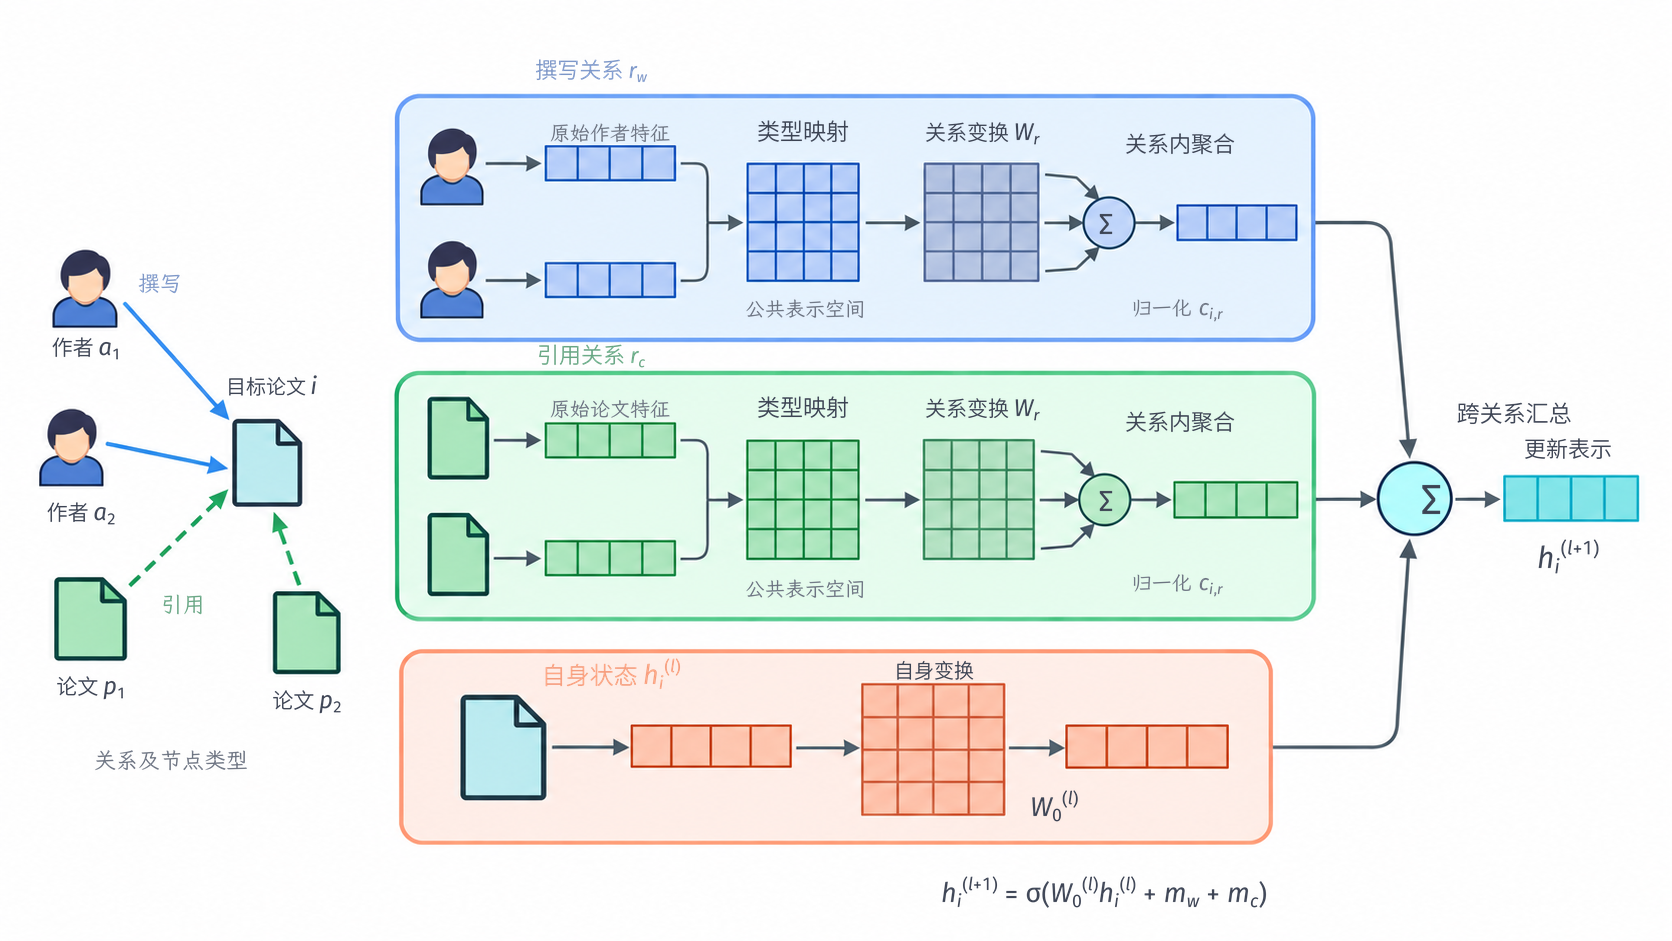
\includegraphics[width=\linewidth]{figures/03-models/02-neural-network-models/generated/gnn-typed-relations/figure.png}
  \caption{两类节点与两种关系的消息组织。作者的撰写关系和论文的引用关系分别经过类型映射与关系变换，再在各关系内部归一化聚合；两路结果$\bm m_{\mathrm w}$、$\bm m_{\mathrm c}$与独立的自身状态路径汇总，形成目标论文的新表示。各类型的特征组表示同类节点，不表示提前求和；矩阵网格只示意变换，不声明实际维度。}
  \label{fig:gnn-typed-relations}
\end{figure*}

\subsection{动态图}
\label{sec:gnn-dynamic}

社交互动、交易和设备关系会随时间改变。\term{动态图}（dynamic graph）把节点、边或属性的变化作为输入的一部分，模型不仅要处理当前关系，还要确定哪些历史在预测时可见。固定图上的十轮传播仍是同一个输入的十次内部计算，与现实中经过十个观测时刻不同。

一种表示是\term{图快照}（graph snapshot）：在时刻$t$取得$\mathcal{G}_t$与$\bm{X}_t$，先在每张快照中编码，再沿时间更新。对持续存在的节点可写为
\begin{equation}
  \bm{z}_{i,t}=\operatorname{GNN}(\mathcal{G}_t,\bm{X}_t)_i,
  \qquad
  \bm{s}_{i,t}=\operatorname{GRU}(\bm{s}_{i,t-1},\bm{z}_{i,t})\text{。}
  \label{eq:gnn-snapshot-dynamics}
\end{equation}
这里$\bm{z}_{i,t}$包含当前图中的邻域信息，$\bm{s}_{i,t}$维护跨时间历史。节点身份用于对齐相邻快照中的同一个对象；新节点的初态、节点消失后的状态保留与重现规则也要约定。快照间隔决定哪些短时事件被合并或遗漏。

另一种表示是带时间戳的\term{事件序列}（event sequence），例如第$q$个事件$(i_q,j_q,\tau_q,\bm{a}_q)$表示两个节点在时刻$\tau_q$发生互动。每个节点维护自己的记忆，在事件发生后更新相关状态。消息可以读取两端的事件前记忆、事件属性，以及距离该节点上次更新的时间间隔；不参与事件的节点记忆可以暂时保留。TGN以消息函数、消息聚合、记忆更新和时序表示等模块组织这一类计算\scite{rossi2020tgn}

预测互动是否发生时，应先用事件发生前的历史评分，再用实际发生的事件更新记忆。若把待预测互动写入邻接关系或记忆后才评分，答案已经成为输入。批量事件处理也要明确是否能读取同批中较早的事件；同一时刻的事件若没有已知顺序，不能随意用存储次序制造先后依赖。

图~\ref{fig:gnn-dynamic-before-update}把内部传播、观测时间与事件先后三种顺序分开。下半部的评分位于消息和记忆更新之前，正是避免把待预测事件提前写入历史的关键。

\begin{figure*}[htbp]
  \centering
  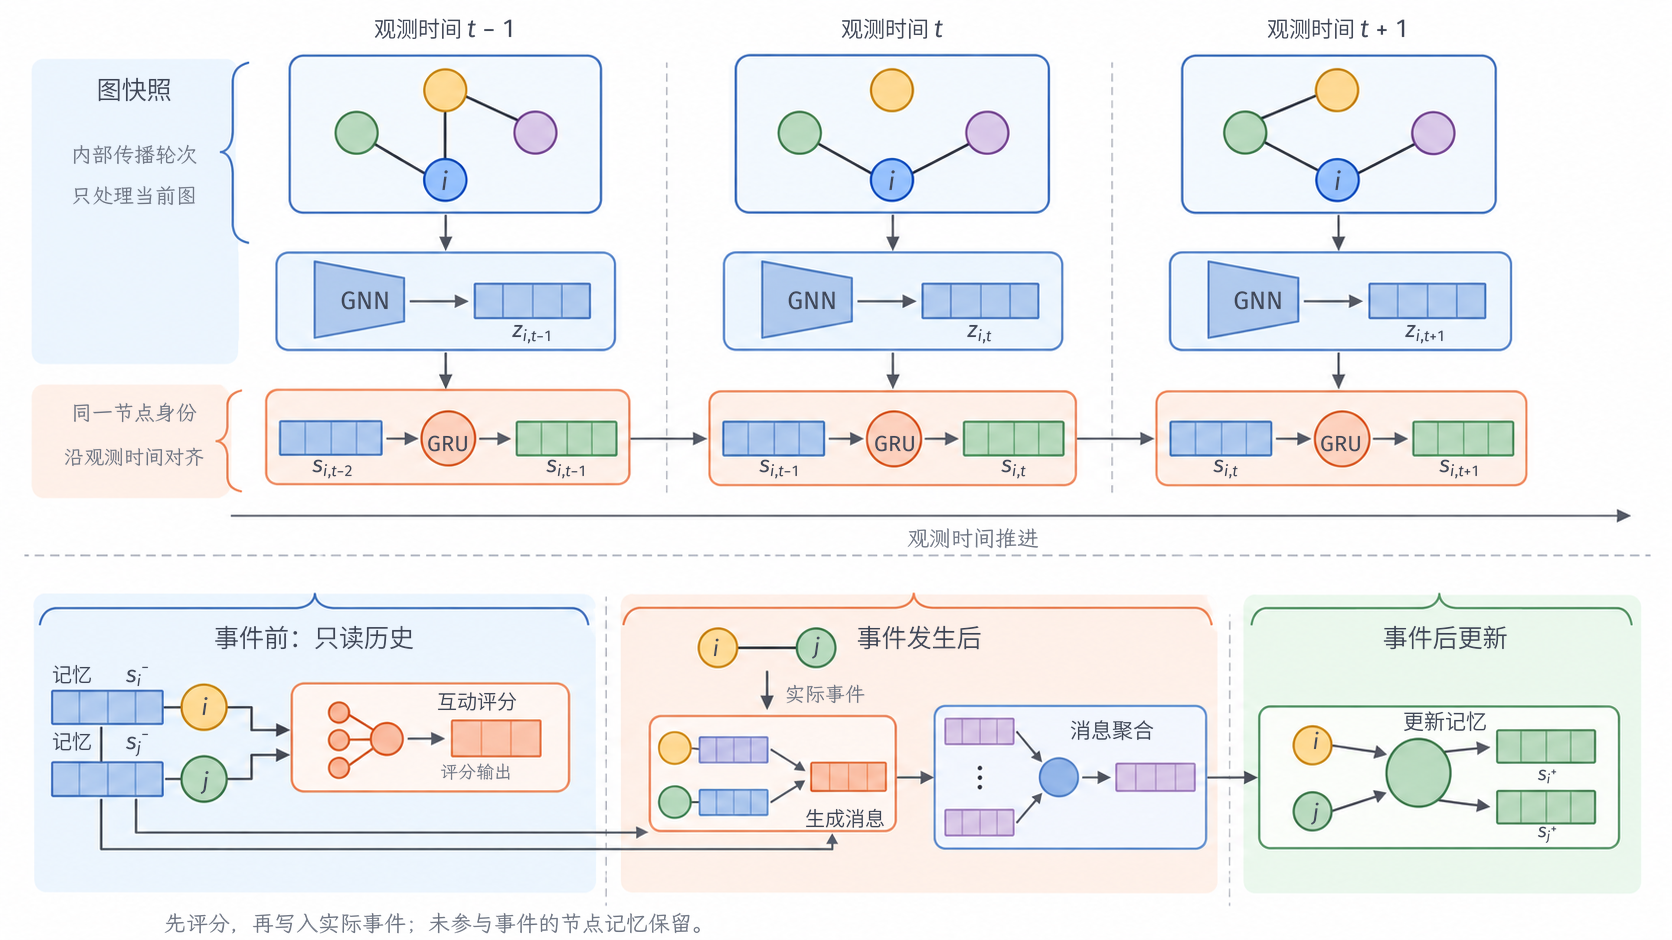
\includegraphics[width=\linewidth]{figures/03-models/02-neural-network-models/generated/gnn-dynamic-before-update/figure.png}
  \caption{动态图的两种时间组织。上半部区分固定快照中的内部传播与同一节点沿观测时间的GRU状态演化；下半部先用事件前记忆评分，实际事件到达后才生成消息、聚合并更新参与节点。未参与事件的节点保留记忆。}
  \label{fig:gnn-dynamic-before-update}
\end{figure*}

训练时可沿快照或事件展开反向传播，并在长流中按需要截断。评估未来事件时按时间划分，状态只由约定的可见历史推进；评估新节点时还要额外检查训练阶段是否已经接触其信息。内部传播深度、历史记忆长度和观测时间间隔共同影响计算，但衡量的是三种不同范围。

\subsection{高阶关系}
\label{sec:gnn-higher-order}

一次多人合作对应一个参与者集合，单条普通边只能描述两个对象。\term{超图}（hypergraph）用\term{超边}（hyperedge）表示同时连接多个节点的关系。记$\mathcal{H}=(V,\mathcal{E})$，其中$\mathcal{E}$是节点子集的集合；一条超边$S_a\subseteq V$保留这次关系的完整参与组。将它拆成所有成对边，可能无法区分“一次三人合作”与“三次两人合作”。

图~\ref{fig:gnn-hyperedge}展示一种计算表示：先让节点向超边聚合，再让超边把结果传回参与节点。将每条超边作为额外对象，会得到节点与关系对象构成的二部图；超边属性及非线性变换可以放在中间状态上。
\begin{figure*}[htb]
  \centering
  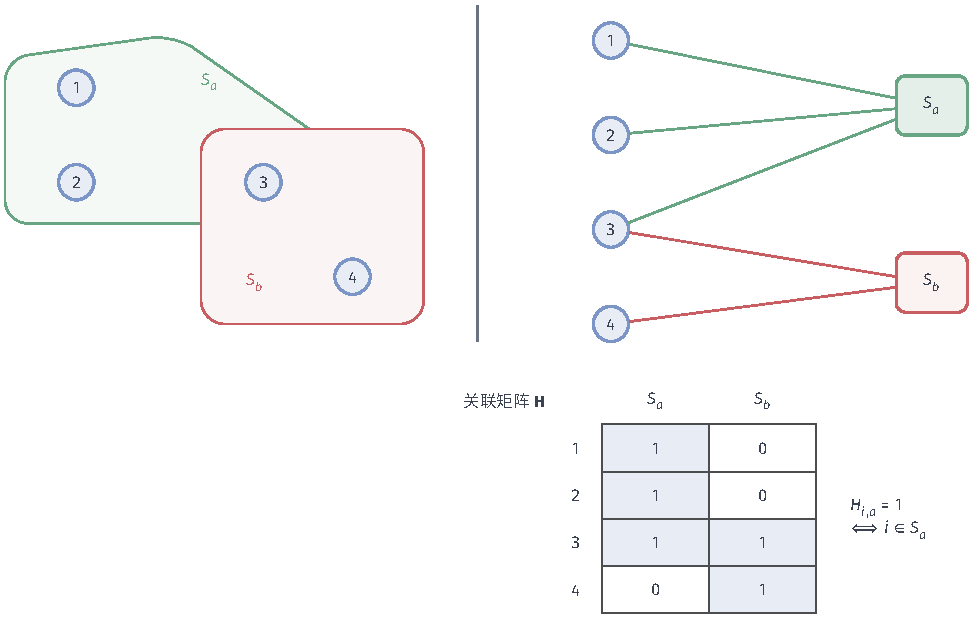
\includegraphics[width=\linewidth]{figures/03-models/02-neural-network-models/tikz/gnn-hyperedge/figure.pdf}
  \caption{超边及其关联表示。左侧一条超边$S_a$连接节点1、2、3，另一条超边$S_b$连接节点3、4。右侧将超边画成方框，以连线表示参与关系；下方$4\times2$关联矩阵$\bm H$用同一组0／1关系把“集合、二部图、矩阵”对应起来。方框是关系状态，不是新增的原始参与者。}
  \label{fig:gnn-hyperedge}
\end{figure*}

令\term{关联矩阵}（incidence matrix）$\bm{B}\in\{0,1\}^{n\times h}$记录节点是否属于超边，$h=|\mathcal{E}|$，$\bm{B}_{i,a}=1$表示$i\in S_a$。设超边权重为$w_a>0$，$\bm{W}_e=\operatorname{diag}(w_1,\ldots,w_h)$，节点度$d_i=\sum_a\bm{B}_{i,a}w_a$，超边大小$s_a=\sum_i\bm{B}_{i,a}$。对非空超边及非孤立节点，一个归一化的传播为
\begin{equation}
  \bm{H}'=\sigma\!\left(
    \bm{D}_v^{-1/2}\bm{B}\bm{W}_e\bm{D}_e^{-1}
      \bm{B}^{\top}\bm{D}_v^{-1/2}\bm{H}\bm{\Theta}\right)\text{，}
  \label{eq:gnn-hypergraph-layer}
\end{equation}
其中$\bm{D}_v=\operatorname{diag}(d_i)$、$\bm{D}_e=\operatorname{diag}(s_a)$，$\bm{\Theta}$是特征变换矩阵。关联矩阵转置把节点信息汇到超边，关联矩阵再将结果送回节点；HGNN采用了这一类归一化超图卷积\scite{feng2019hgnn}

超图输入与更强表达能力仍须区分。式\eqref{eq:gnn-hypergraph-layer}的线性传播部分可以合成一个节点间矩阵，若两张超图产生相同矩阵，这一层也不能保留它们不同的组关系。若任务依赖具体组的区别，需要保留超边状态、属性或组内非线性，不能仅凭输入被称为超图就认定信息已经完整利用。

另一类\term{高阶图网络}（higher-order graph neural network）把节点组作为状态对象，例如为节点对维护$\bm{h}_{i,j}$，使网络能够组合单节点状态难以保留的关系。它不一定需要外部提供超边，而是改变计算状态的索引与交互方式。Morris等将这种思路与高阶WL方法联系起来\scite{morris2019higherorder} 若显式维护所有$k$元节点组，状态数可达$O(n^k)$；选取部分子结构或局部组可以降低代价，但相应的区分能力也要重新说明。

\subsection{几何关系与对称性约束}
\label{sec:gnn-geometric}

原子或物体除了连接关系，还可能具有坐标$\bm{r}_i\in\mathbb{R}^{3}$。若把绝对坐标直接送入普通前馈消息函数，平移或转动物体就可能改变标量属性预测。几何任务需要另外指定对称性：能量等标量通常要求对整体平移和旋转不变；预测的位移或力则应随坐标系一起旋转。

令$\bm{r}'_i=\bm{Q}\bm{r}_i+\bm{t}$，其中$\bm{t}\in\mathbb{R}^{3}$是平移，正交矩阵$\bm{Q}$满足$\bm{Q}^{\top}\bm{Q}=\bm{I}_3$。相对位移随$\bm{Q}$旋转，距离$\lVert\bm{r}_i-\bm{r}_j\rVert_2$保持不变。用距离和其他不变属性产生标量消息，再用标量系数乘相对位移，就能构造等变的坐标更新。一个EGNN式的层可写为
\begin{equation}
  \begin{aligned}
    \bm{m}_{i\leftarrow j}
      &=\phi_e(\bm{h}_i,\bm{h}_j,
        \lVert\bm{r}_i-\bm{r}_j\rVert_2^2,\bm{a}_{i,j}),\\
    \bm{r}'_i&=\bm{r}_i+
      c_i\sum_{j\in N(i)}(\bm{r}_i-\bm{r}_j)\phi_r(\bm{m}_{i\leftarrow j}),\\
    \bm{h}'_i&=\phi_h\!\left(\bm{h}_i,\sum_{j\in N(i)}\bm{m}_{i\leftarrow j}\right)\text{。}
  \end{aligned}
  \label{eq:gnn-egnn}
\end{equation}
$\phi_r$输出标量，$c_i$是与坐标变换无关的归一化系数，$\bm{h}_i$此处由旋转不变的标量通道组成。EGNN使用距离构造消息，并用这种相对位移加权实现欧氏变换等变性\scite{satorras2021egnn}

证明只需跟踪各对象的变化。距离不变，所以消息及$\phi_r$不变；相对位移变为$\bm{Q}(\bm{r}_i-\bm{r}_j)$，整段坐标增量随$\bm{Q}$变换，加回$\bm{Q}\bm{r}_i+\bm{t}$后得到原更新结果的同一变换。邻接构造也须遵守该对称性，例如按距离阈值建边；若按固定坐标轴上的绝对位置选边，消息函数对称仍不足以保证整个模型对称。

正交矩阵还包括镜像反射。距离不变的模型因此可能无法区分互为镜像的手性构型；若目标会因镜像而改变，就需要只约束适用的对称群，并引入能保留相应方向关系的信息。对称性必须来自任务，不能为了方便把本该保留的差别抹掉。

若标量能量预测$\widehat E$可微且具有相应不变性，定义$\widehat{\bm{f}}_i=-\nabla_{\bm{r}_i}\widehat E$可以得到随旋转等变的力预测。这个构造保证输出间的数学一致性，却不保证学到的能量或力具有足够精度；仍需合适监督、结构覆盖及数值计算。

\section{理论分析}
\label{sec:gnn-theory}

图结构改变了信息的传播路径，也改变了训练数据的依赖方式。讨论理论性质时，需要明确是在固定参数下计算状态、比较输入表示，还是从有限样本学习参数。一个层面的良好性质不能直接替代另一个层面的保证。

\subsection{收敛与信息传播}
\label{sec:gnn-propagation-theory}

\subsubsection{状态收敛及其条件}
\label{sec:gnn-state-convergence}

不动点模型需要知道反复更新是否会停在确定的状态。使用卷一的\term{压缩映射}（contraction mapping）条件：对同一输入，两份状态经过更新后距离按小于1的固定比例缩小。这里的距离针对整张图的状态，不能只检查单个节点的激活函数。

\begin{theorem}[压缩更新的唯一不动点]
\label{thm:gnn-contraction}
固定$\mathcal{G}$、$\bm{X}$和参数$\bm{\theta}$。设$F_{\bm{\theta}}$把非空闭状态域$\bm{S}_{\mathrm{state}}\subseteq\mathbb{R}^{nm}$映到自身，且某个范数下存在$c\in[0,1)$，使任意$\bm{u},\bm{v}\in\bm{S}_{\mathrm{state}}$满足
\[
  \lVert F_{\bm{\theta}}(\bm{u})-F_{\bm{\theta}}(\bm{v})\rVert
    \leq c\lVert\bm{u}-\bm{v}\rVert\text{。}
\]
则$\bm{S}_{\mathrm{state}}$中存在唯一不动点$\bm{h}^*$，任意该域内初态的迭代都收敛到它，并满足
\begin{equation}
  \lVert\bm{h}^{(t)}-\bm{h}^*\rVert
    \leq c^t\lVert\bm{h}^{(0)}-\bm{h}^*\rVert\text{。}
  \label{eq:gnn-contraction-error}
\end{equation}
\end{theorem}
\begin{proof}
应用\BookTheoremRef{thm:analysis-banach-fixed-point}{第一卷“数学准备”的Banach不动点定理}。
闭状态域在有限维范数下完备，自映射与统一压缩条件保证状态极限及其唯一性。
\end{proof}

卷一的后验误差界还给出可检查的状态误差证书：对$t\geq1$，$\lVert\bm{h}^{(t)}-\bm{h}^*\rVert\leq c(1-c)^{-1}\lVert\bm{h}^{(t)}-\bm{h}^{(t-1)}\rVert$。$c$接近1时，相邻差小不代表离不动点已经同样近；迭代速度和停止容差要放在一起解释。

例如采用矩阵状态更新$\bm{H}'=\sigma(\bm{S}\bm{H}\bm{W}+\bm{B}_x)$，其中$\bm{B}_x\in\mathbb{R}^{n\times m}$为固定输入项。若$\sigma$是$L_\sigma$-Lipschitz的，则Frobenius范数下
\begin{equation}
  \lVert\bm{H}'_1-\bm{H}'_2\rVert_F
    \leq L_\sigma\lVert\bm{S}\rVert_2\lVert\bm{W}\rVert_2
      \lVert\bm{H}_1-\bm{H}_2\rVert_F\text{。}
  \label{eq:gnn-state-lipschitz}
\end{equation}
乘积小于1且状态域不变时，可应用定理。未经归一化的求和传播可能因最大节点度增大而放大该上界；对称归一化的无向GCN传播满足$\lVert\bm{S}\rVert_2=1$。门控中的门值落在$[0,1]$仍不足以单独保证收缩，因为门自身也随状态变化。

收缩保证的是固定参数下的状态计算。参数更新会改变$F_{\bm{\theta}}$，整个训练目标通常仍然非凸；收敛到状态不动点不等于参数优化收敛，更不等于训练或测试损失小。收缩也是充分条件而非必要条件，有限轮次模型本来就不要求以不动点定义输出。

\subsubsection{过平滑：节点区分信息消失}
\label{sec:gnn-oversmoothing}

传播扩大感受野，却可能把不同节点的表示反复混在一起。\term{过平滑}（oversmoothing）指传播加深后，与节点差异有关的信息不断减少，以致任务需要的区分难以保留。它可以发生在没有循环共享参数的深层网络中，也不要求所有坐标在字面上完全相等。

\begin{figure}[htbp]
  \centering
  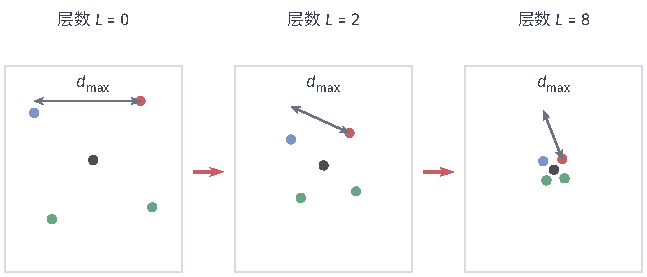
\includegraphics[width=\linewidth]{figures/03-models/02-neural-network-models/tikz/gnn-oversmoothing/figure.pdf}
  \caption{过平滑的二维投影示意。五种颜色始终代表同五个节点，位置只是人为构造的表示投影，并非t-SNE实验；随着传播层数增加，点间最大距离缩小，节点身份仍在但可供下游区分的表示差异逐渐消失。过平滑描述的是任务相关差异受损，不要求所有坐标严格相等。}
  \label{fig:gnn-oversmoothing}
\end{figure}

先看一个能够精确求解的简化模型：令激活与通道变换都为恒等，只反复计算$\bm{H}^{(l+1)}=\bm{S}\bm{H}^{(l)}$。假定非负无向图连通，并在每个节点加入正自环；对应$\bm{S}$具有唯一特征值1，其余特征值的绝对值小于1。定义单位向量
\[
  q_i=\frac{\sqrt{\widetilde d_i}}{\sqrt{\sum_j\widetilde d_j}}\text{，}
\]
则特征分解给出
\begin{equation}
  \bm{S}^L\bm{X}\longrightarrow\bm{q}\bm{q}^{\top}\bm{X},\qquad
  \lVert\bm{S}^L\bm{X}-\bm{q}\bm{q}^{\top}\bm{X}\rVert_F
    \leq\rho^L\lVert\bm{X}\rVert_F\text{，}
  \label{eq:gnn-linear-oversmoothing}
\end{equation}
其中$\rho$是其他特征值绝对值的最大值。证明依据是$\bm{q}$方向保持不变，其正交方向每次乘以绝对值至多为$\rho$的特征值。

极限中，每个节点只剩同一个特征向量的度相关倍数；除以$\sqrt{\widetilde d_i}$后便相同。若图不连通，每个连通分量保留一个相应方向；若没有破除周期的条件，例如无自环的二部图，状态还可能振荡。因而连通性、归一化与自环都是结论的条件，不能省略。

真实GCN还含非线性、学习权重与跨层连接，不能直接把式\eqref{eq:gnn-linear-oversmoothing}视为它们的全部行为。Oono与Suzuki在特定激活及参数范数条件下进一步分析了表示靠近低维子空间的速度，说明传播谱与权重尺度需要联合考察\scite{oono2020oversmoothing} 低频聚合在有限深度可能有用，任务需要保留的差异被过度削弱时才构成问题。

残差连接可以为旧表示保留额外路径，跨层拼接或读出可以直接读取较浅表示，初始特征注入则持续补充原始节点差异。这些设计改变了反复纯混合的形式。仅给传播加一个恒等分支后再归一化，仍可能逐步混合，因此不能只凭出现“残差”就认定过平滑已经消失。

\subsubsection{过压缩：远处信息通过狭窄通路}
\label{sec:gnn-oversquashing}

另一种困难是节点需要利用许多远处对象，但这些信息只能经少量中间状态到达。\term{过压缩}（oversquashing）指大量关系信息沿传播路径汇入有限维状态或狭窄连接时，任务所需的远处影响难以有效传递。它关注路径与容量，而不是节点表示是否趋同；Alon与Yahav从这一信息瓶颈出发分析了长程图任务\scite{alon2021oversquashing}

一个二叉树例子能展示具体机制。设每个内部节点只把两个子节点的标量取平均，深度为$k$的$2^k$个叶子为$x_j$，则根状态为$h_{\mathrm{root}}=2^{-k}\sum_jx_j$，对单个叶子的导数为$2^{-k}$。距离增加时，每个叶子的单独影响迅速衰减；但根与各叶状态并没有被要求相同。图~\ref{fig:gnn-bottleneck}将汇聚树与图中的狭窄连接对应起来。

\begin{figure*}[htb]
  \centering
  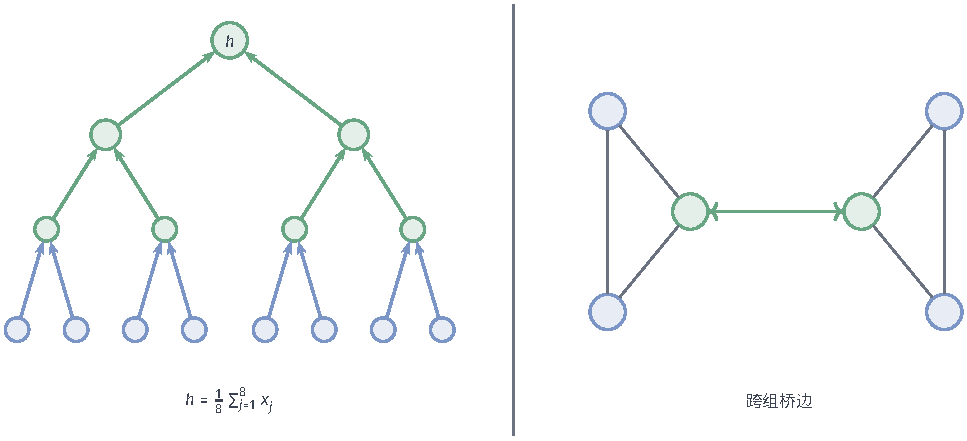
\includegraphics[width=\linewidth]{figures/03-models/02-neural-network-models/tikz/gnn-bottleneck/figure.pdf}
  \caption{两种信息汇聚瓶颈。左侧八个叶子经三层平均进入一个根状态，每个叶子的影响系数为$1/8$；右侧两组节点的跨组信息必须经过一条桥边。红色表示承担汇聚或跨组传递的状态，蓝色表示外围输入。图不要求所有状态相同，强调的是大量信息必须经过较少的表示通路。}
  \label{fig:gnn-bottleneck}
\end{figure*}

若目标恰是叶子的平均，这种压缩就是所需计算；若目标要根据查询分别检索某个叶子，单一平均已经丢掉必要差别。因此，过压缩要相对于任务解释。有限维实数在无限精度下还可能编码大量离散信息，不能只凭维度给出不带连续性、噪声或有限精度条件的绝对存储不可能性结论。

增加状态宽度可以提供更多通道，增加传播轮次可以到达更远处，却也可能增加汇入同一状态的信息量。修改图结构、加入长程连接或全局读取，可以缩短路径并扩大跨区域通路；这些做法也改变了关系假设和计算量。残差主要保留已有信息路径，未必能解除一条桥边上的瓶颈。状态收敛、过平滑与过压缩因而需要分别诊断，再选择对应设计。

\subsection{泛化能力}
\label{sec:gnn-generalization}

\subsubsection{样本单位与图上的依赖}
\label{sec:gnn-sample-units}

对分子属性预测，一张分子图及其标签可以作为一个样本，图内节点允许相互依赖。若$N$张图独立同分布，前面学习理论中的样本量就是$N$，并不是所有原子数的总和。若多张图来自同一系统的连续快照，或由一张大图截取重叠片段，它们未必独立。

单张引用图上的节点分类具有另一种组织方式：输入结构与特征可以共享，节点标签及其邻域又相互关联。随机选若干标签做训练，并不把全部节点变成独立同分布图样本。固定图上的未标记节点风险可以采用直推分析；从一个图生成模型抽样时，需要把相应结构依赖写进假设。不能把独立样本界中的分母直接改成节点数，就声称相关性已经得到处理。

同样，邻域互不重叠也不自动保证样本独立，可能仍有共同的生成因素。样本划分应对应未来使用：已知图上的剩余标签、全新图、全新节点和未来事件分别有不同的信息边界。比较不同模型时，必须固定这一边界。

\subsubsection{输入尺度、度与参数范数}
\label{sec:gnn-norm-generalization}

在独立整图设定下，结构怎样进入泛化分析，可以先从网络敏感度考察。考虑无偏置层$\bm{H}^{(l+1)}=\sigma(\bm{S}\bm{H}^{(l)}\bm{W}^{(l)})$，激活为1-Lipschitz且零点取零。对同一图上的两份特征，固定参数后有
\begin{equation}
  \lVert\bm{H}^{(L)}-\widetilde{\bm{H}}^{(L)}\rVert_F
    \leq\lVert\bm{S}\rVert_2^L
      \prod_{l=0}^{L-1}\lVert\bm{W}^{(l)}\rVert_2
      \lVert\bm{X}-\widetilde{\bm{X}}\rVert_F\text{。}
  \label{eq:gnn-feature-sensitivity}
\end{equation}
每层先用激活的Lipschitz性，再用矩阵乘法的范数界，逐层相乘即得。它控制固定结构下的输入扰动；若边同时改变，还必须增加传播算子变化的项。

未经归一化的邻接求和在无向图上满足$\lVert\bm{A}\rVert_2\leq d_{\max}$，其中$d_{\max}$是最大加权度。这个上界可能随深度以$d_{\max}^L$进入敏感度；标准对称归一化将传播的谱范数控制为1。归一化因而可以改变尺度控制，但也改变了度与计数信息，不能只根据范数界判断哪种模型在所有任务上更好。

读出又带来规模差别。平均读出满足$\lVert n^{-1}\bm{1}^{\top}\bm{H}\rVert_2\leq\lVert\bm{H}\rVert_F/\sqrt n$，求和读出的对应系数为$\sqrt n$。若每个节点输入范数不超过$B_x$，则$\lVert\bm{X}\rVert_F\leq B_x\sqrt n$；平均与求和对应的输出上界分别消去或保留节点规模。宽度、偏置、注意力评分和关系参数还会改变其余常数，需按实际模型计入。

对权重扰动也可逐层计算。只改变第$k$层权重时，当前误差至多为$\lVert\bm{S}\rVert_2\lVert\bm{H}^{(k)}\rVert_F\lVert\Delta\bm{W}^{(k)}\rVert_2$，后续层再乘各自的尺度界。逐个替换所有层并用三角不等式，可以建立输出对全部参数的统一Lipschitz上界。深度影响重复传播和误差累积，参数共享限制自由度，却不取消同一参数反复使用的敏感度。

\subsubsection{从参数约束到风险界}
\label{sec:gnn-risk-bound}

敏感度还不是泛化结论；需要结合样本抽样和受约束的候选函数族。下面给出一个便于检查条件的整图预测界，承接统计学习部分的一致收敛思路，不假定独立节点。

\begin{theorem}[有界参数图预测的覆盖界]
\label{thm:gnn-cover-generalization}
设$Z_1,\ldots,Z_N$是独立同分布的整图及标签样本。预先固定的参数域$\bm{\Theta}\subseteq\mathbb{R}^{p}$包含在半径$B_\theta>0$的欧氏球内，损失$\ell_{\bm{\theta}}(Z)\in[0,1]$关于样本可测，且对全部允许的样本与参数有
\[
  |\ell_{\bm{\theta}}(Z)-\ell_{\widetilde{\bm{\theta}}}(Z)|
    \leq a\lVert\bm{\theta}-\widetilde{\bm{\theta}}\rVert_2
\]
其中$a>0$为预先给定的统一常数。记期望风险$R(\bm{\theta})=\mathbb{E}\ell_{\bm{\theta}}(Z)$与经验风险$\widehat R_N(\bm{\theta})=N^{-1}\sum_q\ell_{\bm{\theta}}(Z_q)$。对任意预先固定的$\varepsilon>0$与$\delta\in(0,1)$，以至少$1-\delta$的概率，
\begin{equation}
  \begin{aligned}
    \sup_{\bm{\theta}\in\bm{\Theta}}
      |R(\bm{\theta})-\widehat R_N(\bm{\theta})|
      &\leq2\varepsilon\\
      &\quad+\sqrt{\frac{p\log(1+2B_\theta a/\varepsilon)
        +\log(2/\delta)}{2N}}\text{。}
  \end{aligned}
  \label{eq:gnn-cover-risk}
\end{equation}
\end{theorem}
\begin{proof}
欧氏球内的参数集合有半径$\varepsilon/a$的覆盖，中心取自$\bm{\Theta}$，覆盖数至多为$(1+2B_\theta a/\varepsilon)^p$。对每个中心的有界损失使用Hoeffding不等式，再用并合界，得到平方根项。任意参数到最近中心的损失差不超过$\varepsilon$，期望风险与经验风险各增加至多$\varepsilon$，合计得到$2\varepsilon$。
\end{proof}

这个界把独立图数、参数自由度、参数范围和统一敏感度放在同一表达式中。前面的范数推导可以在限定图规模、特征尺度与网络结构后帮助构造$a$；图拓扑及度会通过传播算子进入它。假设对全部允许样本成立很关键：仅在训练图上测到较小梯度，不足以建立同样的统一覆盖保证。

原始交叉熵无上界，不能直接代入$[0,1]$条件；可使用有界替代损失，或在额外概率下界及尺度处理后重新分析。这个参数覆盖界也可能很松，它展示的是一条充分条件路线，而不是精确预测测试误差的公式。Rademacher复杂度可以更细地利用样本和函数约束，算法稳定性则研究替换一个完整图样本后学习结果的变化；采用哪一种工具，都必须与样本单位和损失条件对应。

结构设计还影响拟合偏差。更强的对称性减少无关自由度，却可能排除任务需要的方向差异；更强的聚合区分能力扩大可表达的函数，也需要数据与学习过程支持。残差提供额外路径时，其Lipschitz上界常出现$1+$分支尺度，不能因为梯度路径改善就宣称复杂度界一定降低。

测试图比训练图更大、节点度分布不同，或关系类型及标签机制变化时，已经改变了输入分布。共享更新可以在新规模上执行，仍不保证超出训练范围的误差保持不变。应分别报告同分布整图泛化、固定图直推表现及跨规模或跨分布结果，把结构优势与数据条件放在一起解释。

\section{常见应用}
\label{sec:gnn-applications}

以下三个任务使用不同预测对象，但都需要把可见关系、编码器、输出和监督对应起来。具体领域的特征工程、评估协议和应用方法留给应用卷，这里展示一个完整模型如何接入任务。

\subsection{节点分类}
\label{sec:gnn-application-node}

以论文引用网络为例，每篇论文是节点，内容向量是$\bm{x}_i$，引用是有向边。若任务允许同时读取引用与被引用的信息，可以分别使用两个方向，或明确把图无向化；后一种选择会丢掉方向差别。内容编码器只使用约定的可见文本，类别标签另放在监督集合中。

一个基本模型是两层GCN：$\bm{H}^{(1)}=\operatorname{ReLU}(\bm{S}\bm{X}\bm{W}^{(0)})$，节点概率矩阵为$\bm{P}=\operatorname{softmax}_{\mathrm{row}}(\bm{S}\bm{H}^{(1)}\bm{W}^{(1)})$，Softmax逐行作用。按式\eqref{eq:gnn-node-loss}仅在训练节点上计算交叉熵，反向更新两层权重。两轮传播使每个预测可以读取两跳以内的内容与连接信息。

直推设定下，验证和测试节点的无标签特征与连接可以按协议参与编码；类别标签用于各自的评估，不能进入训练计算。若预测未来发表的论文，则训练时不得使用未来引用边和文本，内容编码、建图及归一化也须按当时可见的信息重建。相同两层公式可以用于两种设定，但它们回答的是不同泛化问题。

还应比较只使用内容的前馈基线，以检查关系是否提供了额外信息。邻居类别常相近时聚合可能有用；关系跨越类别边界时，需要分开自身与邻居、处理方向或关系类型，不能预设相邻论文属于同类。

\subsection{连接预测}
\label{sec:gnn-application-link}

关系网络中，编码器先在可见图上产生$\bm{z}_i=\bm{h}_i^{(L)}$，解码器再为候选节点对评分。无向连接可用$s_{i,j}=\bm{z}_i^{\top}\bm{z}_j$；有向关系可用$s_{i,j}=\bm{z}_i^{\top}\bm{R}\bm{z}_j$，一般矩阵$\bm{R}$允许交换端点后得分变化。多关系任务可把$\bm{R}$改为类型相关参数。

训练批次包含已知正连接及从候选范围抽出的负样本，按式\eqref{eq:gnn-edge-loss}联合更新编码器与评分参数。未观察到的边并不一定是真实负例，它可能只是尚未记录；采样范围、正负比例和缺失机制决定目标的含义。以人为采样比例训练的Sigmoid得分，也不能未经校准就当作现实连接概率。

评估保留连接时，需要从编码图中移除这些边及其反向副本，避免编码器直接读取答案。训练正边是否在给该边评分时仍参与编码，也应说明；可以另外划分用于消息传递与用于监督的正边，或在批次中临时屏蔽目标边，使训练输入与目标评估口径对应。对未来连接，则先用历史图评分，事件发生后再更新动态图状态。

预测时对所需候选评分和排序。全部节点对数量为$O(n^2)$，即使编码器在稀疏图上计算，枚举全部候选仍可能昂贵。候选生成与负样本改变评价难度，比较模型时需要固定它们；容易的随机负例上的高分不代表已解决实际候选中的关系判断。

\subsection{整图属性预测}
\label{sec:gnn-application-graph}

以分子属性预测为例，节点表示原子，边表示化学键。原子种类、形式电荷等作为节点属性，键类型等作为边属性，消息函数据此产生固定宽度向量。传播若干轮后，通过式\eqref{eq:gnn-readout}形成分子表示，再用前馈输出头预测标量，按式\eqref{eq:gnn-graph-loss}学习。输入编码、消息函数、更新与输出头共同接受梯度。

读出选择要与属性性质对应。随体系大小累积的量可以采用节点贡献求和的结构，强调整体分子组成；与规模不直接成比例的量可以使用平均或更一般的可学习读出。真实属性是否可由局部贡献充分表达仍取决于任务，不能把求和形式直接当作物理正确性的保证。

只有二维连接关系时，网络不知道同一分子不同空间构型的坐标差别。若目标依赖三维构型，需要把预测时可得的坐标与几何关系纳入，并按第~\ref{sec:gnn-geometric}节处理对称性。近邻空间图与化学键图还可以承担不同关系通路，不能将二者的边含义混同。

训练和测试按完整分子划分；同一分子的多种构型或高度相近的结构是否跨划分，需要与目标使用场景对应。仅随机分图可能主要检查近似结构间的插值，按结构族划分则考察更远的迁移。验证图用于选择传播深度、宽度与读出，测试图用于评价相应设定下的预测误差。

\section{本章小结}
\label{sec:gnn-summary}

图神经网络沿关系传递信息，用共享消息与对称聚合处理数量不定、次序无关的邻域。节点表示随重编号等变，整图读出对重编号不变。多轮传播扩大可见范围，聚合、状态宽度与拓扑则共同决定能否保留任务需要的信息。

谱域滤波通过多项式转为局部传播，GCN体现了它与空域聚合的联系。采样、内容加权和多重集合区分解决不同问题；循环共享则须区分有限展开与不动点求解。关系类型、时间、高阶关系和几何对称性进一步规定了哪些信息必须保留。

状态梯度沿前向读取反向回传，并汇合为共享参数的导数；训练趋于驻点需要目标、梯度估计与步长满足相应条件。固定参数的状态收敛保证求值，过平滑描述节点差异消失，过压缩描述远处信息受到狭窄通路限制。建模时须确定可见关系与适用对称性，选择任务读出，再用匹配的监督和划分检验。结构能够在新图上执行是起点，可靠性仍须结合样本依赖、图分布与参数尺度考察。
